% This must be in the first 5 lines to tell arXiv to use pdfLaTeX, which is strongly recommended.
\pdfoutput=1
% In particular, the hyperref package requires pdfLaTeX in order to break URLs across lines.

\documentclass[11pt]{article}
% \usepackage[table]{xcolor} % Include the xcolor package

% Remove the "review" option to generate the final version.
\usepackage[]{style/acl}

% Standard package includes
\usepackage{times}
\usepackage{latexsym}
\usepackage{multirow}
% For proper rendering and hyphenation of words containing Latin characters (including in bib files)
\usepackage[T1]{fontenc}
% For Vietnamese characters
% \usepackage[T5]{fontenc}
% See https://www.latex-project.org/help/documentation/encguide.pdf for other character sets

\usepackage{amsmath}
\usepackage{verbatim}
\usepackage{paralist}
% This assumes your files are encoded as UTF8
\usepackage[utf8]{inputenc}

% This is not strictly necessary, and may be commented out.
% However, it will improve the layout of the manuscript,
% and will typically save some space.
\usepackage{microtype}

% This is also not strictly necessary, and may be commented out.
% However, it will improve the aesthetics of text in
% the typewriter font.
\usepackage{inconsolata}
\usepackage{soul}

\usepackage{booktabs}
\usepackage{graphicx}
\usepackage[export]{adjustbox}
\usepackage{soul}
\usepackage{xcolor}

% \newcommand{\hlg}[1]{\sethlcolor{green}\hl{#1}\sethlcolor{yellow}}
\newcommand{\hlg}[1]{#1}
\renewcommand{\hl}[1]{#1}

\usepackage{soulpos} % Extended version of `soul` for nested commands
\usepackage{etoolbox}
\newcommand{\role}[1]{\textsc{#1}}
% \newcommand{\tbd}[1]{\marginpar{\footnotesize#1}}
\newcommand{\tbd}[1]{}

\usepackage{colortbl}
\usepackage{pgfplots}

\usepackage{tabularx}
\usepackage{icomma}
% If the title and author information does not fit in the area allocated, uncomment the following
%
%\setlength\titlebox{<dim>}
%
% and set <dim> to something 5cm or larger.

\title{
  Making Language Models Robust Against Negation
}

\author{MohammadHossein Rezaei \and Eduardo Blanco \\
         Department of Computer Science, University of Arizona \\ \texttt{\{mhrezaei,eduardoblanco\}@arizona.edu}}

% \pagecolor{yellow!20}
\begin{document}
\maketitle
\begin{abstract}
Negation has been a long-standing challenge for language models.
Previous studies have shown that they struggle with negation in many natural language understanding tasks.
In this work, we propose a self-supervised method to make language models more robust against negation.
We introduce a novel task, Next Sentence Polarity Prediction (NSPP), and a variation of the Next Sentence Prediction (NSP) task.
We show that BERT and RoBERTa further pre-trained on our tasks outperform the off-the-shelf versions on nine negation-related benchmarks.
Most notably, our pre-training tasks yield between 1.8\% and 9.1\% improvement on CondaQA, a large question-answering corpus requiring reasoning over negation.
\end{abstract}


\section{Introduction}
\label{sec:introduction}
The business processes of organizations are experiencing ever-increasing complexity due to the large amount of data, high number of users, and high-tech devices involved \cite{martin2021pmopportunitieschallenges, beerepoot2023biggestbpmproblems}. This complexity may cause business processes to deviate from normal control flow due to unforeseen and disruptive anomalies \cite{adams2023proceddsriftdetection}. These control-flow anomalies manifest as unknown, skipped, and wrongly-ordered activities in the traces of event logs monitored from the execution of business processes \cite{ko2023adsystematicreview}. For the sake of clarity, let us consider an illustrative example of such anomalies. Figure \ref{FP_ANOMALIES} shows a so-called event log footprint, which captures the control flow relations of four activities of a hypothetical event log. In particular, this footprint captures the control-flow relations between activities \texttt{a}, \texttt{b}, \texttt{c} and \texttt{d}. These are the causal ($\rightarrow$) relation, concurrent ($\parallel$) relation, and other ($\#$) relations such as exclusivity or non-local dependency \cite{aalst2022pmhandbook}. In addition, on the right are six traces, of which five exhibit skipped, wrongly-ordered and unknown control-flow anomalies. For example, $\langle$\texttt{a b d}$\rangle$ has a skipped activity, which is \texttt{c}. Because of this skipped activity, the control-flow relation \texttt{b}$\,\#\,$\texttt{d} is violated, since \texttt{d} directly follows \texttt{b} in the anomalous trace.
\begin{figure}[!t]
\centering
\includegraphics[width=0.9\columnwidth]{images/FP_ANOMALIES.png}
\caption{An example event log footprint with six traces, of which five exhibit control-flow anomalies.}
\label{FP_ANOMALIES}
\end{figure}

\subsection{Control-flow anomaly detection}
Control-flow anomaly detection techniques aim to characterize the normal control flow from event logs and verify whether these deviations occur in new event logs \cite{ko2023adsystematicreview}. To develop control-flow anomaly detection techniques, \revision{process mining} has seen widespread adoption owing to process discovery and \revision{conformance checking}. On the one hand, process discovery is a set of algorithms that encode control-flow relations as a set of model elements and constraints according to a given modeling formalism \cite{aalst2022pmhandbook}; hereafter, we refer to the Petri net, a widespread modeling formalism. On the other hand, \revision{conformance checking} is an explainable set of algorithms that allows linking any deviations with the reference Petri net and providing the fitness measure, namely a measure of how much the Petri net fits the new event log \cite{aalst2022pmhandbook}. Many control-flow anomaly detection techniques based on \revision{conformance checking} (hereafter, \revision{conformance checking}-based techniques) use the fitness measure to determine whether an event log is anomalous \cite{bezerra2009pmad, bezerra2013adlogspais, myers2018icsadpm, pecchia2020applicationfailuresanalysispm}. 

The scientific literature also includes many \revision{conformance checking}-independent techniques for control-flow anomaly detection that combine specific types of trace encodings with machine/deep learning \cite{ko2023adsystematicreview, tavares2023pmtraceencoding}. Whereas these techniques are very effective, their explainability is challenging due to both the type of trace encoding employed and the machine/deep learning model used \cite{rawal2022trustworthyaiadvances,li2023explainablead}. Hence, in the following, we focus on the shortcomings of \revision{conformance checking}-based techniques to investigate whether it is possible to support the development of competitive control-flow anomaly detection techniques while maintaining the explainable nature of \revision{conformance checking}.
\begin{figure}[!t]
\centering
\includegraphics[width=\columnwidth]{images/HIGH_LEVEL_VIEW.png}
\caption{A high-level view of the proposed framework for combining \revision{process mining}-based feature extraction with dimensionality reduction for control-flow anomaly detection.}
\label{HIGH_LEVEL_VIEW}
\end{figure}

\subsection{Shortcomings of \revision{conformance checking}-based techniques}
Unfortunately, the detection effectiveness of \revision{conformance checking}-based techniques is affected by noisy data and low-quality Petri nets, which may be due to human errors in the modeling process or representational bias of process discovery algorithms \cite{bezerra2013adlogspais, pecchia2020applicationfailuresanalysispm, aalst2016pm}. Specifically, on the one hand, noisy data may introduce infrequent and deceptive control-flow relations that may result in inconsistent fitness measures, whereas, on the other hand, checking event logs against a low-quality Petri net could lead to an unreliable distribution of fitness measures. Nonetheless, such Petri nets can still be used as references to obtain insightful information for \revision{process mining}-based feature extraction, supporting the development of competitive and explainable \revision{conformance checking}-based techniques for control-flow anomaly detection despite the problems above. For example, a few works outline that token-based \revision{conformance checking} can be used for \revision{process mining}-based feature extraction to build tabular data and develop effective \revision{conformance checking}-based techniques for control-flow anomaly detection \cite{singh2022lapmsh, debenedictis2023dtadiiot}. However, to the best of our knowledge, the scientific literature lacks a structured proposal for \revision{process mining}-based feature extraction using the state-of-the-art \revision{conformance checking} variant, namely alignment-based \revision{conformance checking}.

\subsection{Contributions}
We propose a novel \revision{process mining}-based feature extraction approach with alignment-based \revision{conformance checking}. This variant aligns the deviating control flow with a reference Petri net; the resulting alignment can be inspected to extract additional statistics such as the number of times a given activity caused mismatches \cite{aalst2022pmhandbook}. We integrate this approach into a flexible and explainable framework for developing techniques for control-flow anomaly detection. The framework combines \revision{process mining}-based feature extraction and dimensionality reduction to handle high-dimensional feature sets, achieve detection effectiveness, and support explainability. Notably, in addition to our proposed \revision{process mining}-based feature extraction approach, the framework allows employing other approaches, enabling a fair comparison of multiple \revision{conformance checking}-based and \revision{conformance checking}-independent techniques for control-flow anomaly detection. Figure \ref{HIGH_LEVEL_VIEW} shows a high-level view of the framework. Business processes are monitored, and event logs obtained from the database of information systems. Subsequently, \revision{process mining}-based feature extraction is applied to these event logs and tabular data input to dimensionality reduction to identify control-flow anomalies. We apply several \revision{conformance checking}-based and \revision{conformance checking}-independent framework techniques to publicly available datasets, simulated data of a case study from railways, and real-world data of a case study from healthcare. We show that the framework techniques implementing our approach outperform the baseline \revision{conformance checking}-based techniques while maintaining the explainable nature of \revision{conformance checking}.

In summary, the contributions of this paper are as follows.
\begin{itemize}
    \item{
        A novel \revision{process mining}-based feature extraction approach to support the development of competitive and explainable \revision{conformance checking}-based techniques for control-flow anomaly detection.
    }
    \item{
        A flexible and explainable framework for developing techniques for control-flow anomaly detection using \revision{process mining}-based feature extraction and dimensionality reduction.
    }
    \item{
        Application to synthetic and real-world datasets of several \revision{conformance checking}-based and \revision{conformance checking}-independent framework techniques, evaluating their detection effectiveness and explainability.
    }
\end{itemize}

The rest of the paper is organized as follows.
\begin{itemize}
    \item Section \ref{sec:related_work} reviews the existing techniques for control-flow anomaly detection, categorizing them into \revision{conformance checking}-based and \revision{conformance checking}-independent techniques.
    \item Section \ref{sec:abccfe} provides the preliminaries of \revision{process mining} to establish the notation used throughout the paper, and delves into the details of the proposed \revision{process mining}-based feature extraction approach with alignment-based \revision{conformance checking}.
    \item Section \ref{sec:framework} describes the framework for developing \revision{conformance checking}-based and \revision{conformance checking}-independent techniques for control-flow anomaly detection that combine \revision{process mining}-based feature extraction and dimensionality reduction.
    \item Section \ref{sec:evaluation} presents the experiments conducted with multiple framework and baseline techniques using data from publicly available datasets and case studies.
    \item Section \ref{sec:conclusions} draws the conclusions and presents future work.
\end{itemize}
\section{RELATED WORK}
\label{sec:relatedwork}
In this section, we describe the previous works related to our proposal, which are divided into two parts. In Section~\ref{sec:relatedwork_exoplanet}, we present a review of approaches based on machine learning techniques for the detection of planetary transit signals. Section~\ref{sec:relatedwork_attention} provides an account of the approaches based on attention mechanisms applied in Astronomy.\par

\subsection{Exoplanet detection}
\label{sec:relatedwork_exoplanet}
Machine learning methods have achieved great performance for the automatic selection of exoplanet transit signals. One of the earliest applications of machine learning is a model named Autovetter \citep{MCcauliff}, which is a random forest (RF) model based on characteristics derived from Kepler pipeline statistics to classify exoplanet and false positive signals. Then, other studies emerged that also used supervised learning. \cite{mislis2016sidra} also used a RF, but unlike the work by \citet{MCcauliff}, they used simulated light curves and a box least square \citep[BLS;][]{kovacs2002box}-based periodogram to search for transiting exoplanets. \citet{thompson2015machine} proposed a k-nearest neighbors model for Kepler data to determine if a given signal has similarity to known transits. Unsupervised learning techniques were also applied, such as self-organizing maps (SOM), proposed \citet{armstrong2016transit}; which implements an architecture to segment similar light curves. In the same way, \citet{armstrong2018automatic} developed a combination of supervised and unsupervised learning, including RF and SOM models. In general, these approaches require a previous phase of feature engineering for each light curve. \par

%DL is a modern data-driven technology that automatically extracts characteristics, and that has been successful in classification problems from a variety of application domains. The architecture relies on several layers of NNs of simple interconnected units and uses layers to build increasingly complex and useful features by means of linear and non-linear transformation. This family of models is capable of generating increasingly high-level representations \citep{lecun2015deep}.

The application of DL for exoplanetary signal detection has evolved rapidly in recent years and has become very popular in planetary science.  \citet{pearson2018} and \citet{zucker2018shallow} developed CNN-based algorithms that learn from synthetic data to search for exoplanets. Perhaps one of the most successful applications of the DL models in transit detection was that of \citet{Shallue_2018}; who, in collaboration with Google, proposed a CNN named AstroNet that recognizes exoplanet signals in real data from Kepler. AstroNet uses the training set of labelled TCEs from the Autovetter planet candidate catalog of Q1–Q17 data release 24 (DR24) of the Kepler mission \citep{catanzarite2015autovetter}. AstroNet analyses the data in two views: a ``global view'', and ``local view'' \citep{Shallue_2018}. \par


% The global view shows the characteristics of the light curve over an orbital period, and a local view shows the moment at occurring the transit in detail

%different = space-based

Based on AstroNet, researchers have modified the original AstroNet model to rank candidates from different surveys, specifically for Kepler and TESS missions. \citet{ansdell2018scientific} developed a CNN trained on Kepler data, and included for the first time the information on the centroids, showing that the model improves performance considerably. Then, \citet{osborn2020rapid} and \citet{yu2019identifying} also included the centroids information, but in addition, \citet{osborn2020rapid} included information of the stellar and transit parameters. Finally, \citet{rao2021nigraha} proposed a pipeline that includes a new ``half-phase'' view of the transit signal. This half-phase view represents a transit view with a different time and phase. The purpose of this view is to recover any possible secondary eclipse (the object hiding behind the disk of the primary star).


%last pipeline applies a procedure after the prediction of the model to obtain new candidates, this process is carried out through a series of steps that include the evaluation with Discovery and Validation of Exoplanets (DAVE) \citet{kostov2019discovery} that was adapted for the TESS telescope.\par
%



\subsection{Attention mechanisms in astronomy}
\label{sec:relatedwork_attention}
Despite the remarkable success of attention mechanisms in sequential data, few papers have exploited their advantages in astronomy. In particular, there are no models based on attention mechanisms for detecting planets. Below we present a summary of the main applications of this modeling approach to astronomy, based on two points of view; performance and interpretability of the model.\par
%Attention mechanisms have not yet been explored in all sub-areas of astronomy. However, recent works show a successful application of the mechanism.
%performance

The application of attention mechanisms has shown improvements in the performance of some regression and classification tasks compared to previous approaches. One of the first implementations of the attention mechanism was to find gravitational lenses proposed by \citet{thuruthipilly2021finding}. They designed 21 self-attention-based encoder models, where each model was trained separately with 18,000 simulated images, demonstrating that the model based on the Transformer has a better performance and uses fewer trainable parameters compared to CNN. A novel application was proposed by \citet{lin2021galaxy} for the morphological classification of galaxies, who used an architecture derived from the Transformer, named Vision Transformer (VIT) \citep{dosovitskiy2020image}. \citet{lin2021galaxy} demonstrated competitive results compared to CNNs. Another application with successful results was proposed by \citet{zerveas2021transformer}; which first proposed a transformer-based framework for learning unsupervised representations of multivariate time series. Their methodology takes advantage of unlabeled data to train an encoder and extract dense vector representations of time series. Subsequently, they evaluate the model for regression and classification tasks, demonstrating better performance than other state-of-the-art supervised methods, even with data sets with limited samples.

%interpretation
Regarding the interpretability of the model, a recent contribution that analyses the attention maps was presented by \citet{bowles20212}, which explored the use of group-equivariant self-attention for radio astronomy classification. Compared to other approaches, this model analysed the attention maps of the predictions and showed that the mechanism extracts the brightest spots and jets of the radio source more clearly. This indicates that attention maps for prediction interpretation could help experts see patterns that the human eye often misses. \par

In the field of variable stars, \citet{allam2021paying} employed the mechanism for classifying multivariate time series in variable stars. And additionally, \citet{allam2021paying} showed that the activation weights are accommodated according to the variation in brightness of the star, achieving a more interpretable model. And finally, related to the TESS telescope, \citet{morvan2022don} proposed a model that removes the noise from the light curves through the distribution of attention weights. \citet{morvan2022don} showed that the use of the attention mechanism is excellent for removing noise and outliers in time series datasets compared with other approaches. In addition, the use of attention maps allowed them to show the representations learned from the model. \par

Recent attention mechanism approaches in astronomy demonstrate comparable results with earlier approaches, such as CNNs. At the same time, they offer interpretability of their results, which allows a post-prediction analysis. \par


\section{Empowering Language Models Against Negation}
\label{sec:empowering}

We propose a self-supervised method to make LMs more robust against negation.
Our approach is to further pre-train LMs on two tasks that involve negation.
These tasks are the Next Sentence Polarity Prediction (NSPP) task 
and a variation of the well-known Next Sentence Prediction (NSP) task.
None of these tasks require labeled data\hl{;
any text corpora are suitable.}
Also, they are not specific to any domain or downstream task.



\subsection{Next Sentence Polarity Prediction (NSPP)}
\label{sec:nspp}
We introduce NSPP as the task of predicting the polarity of the next sentence given the current sentence.
\hlg{Given} a pair of consecutive sentences, $(S_1, S_2)$, 
the input to the model is only $S_1$, 
and the output is a binary label indicating whether $S_2$ \hlg{includes} any negation cues or not.
For example, consider the following pair of sentences:
\begin{compactitem}
  \item[] $S_1$: \hl{\textit{The weather report showed sunny skies.}}% \textit{``I like apples.''}
  \item[] $S_2$: \hl{\textit{But it didn’t stay that way.}}% \textit{``I don't like oranges.''}
\end{compactitem}
Given only $S_1$,
the model should predict that the following sentence \hlg{includes} negation cues.



\subsection{Next Sentence Prediction (NSP)}
\label{sec:nsp}
NSP is a well-known task in LM pre-training as first introduced by BERT~\cite{devlin-etal-2019-bert}.
The NSP task is to predict whether two sentences are consecutive.
\citet{devlin-etal-2019-bert} (a) used consecutive sentences from Wikipedia as positive examples 
and (b) chose a random sentence from the same article to replace the second sentence \hl{and} create a negative example.

We propose a variation of the NSP task to improve negation understanding.
For a pair of consecutive sentences, $(S_1, S_2)$,
we create the negative pair $(S_1, S_2')$ 
where $S_2'$ is obtained by reversing the polarity of $S_2$. 
That is, if $S_2$ includes negation cues, we remove them, 
and vice versa. 
\subsubsection{Reversing Polarity}
\label{sec:reversing}

We define rules to add and remove negation cues from sentences.
These rules are used to create the negative pairs $(S_1, S_2')$ in the NSP task.
To streamline the process,
we only work with sentences that
\begin{compactitem}
    \item include \emph{not}, \emph{n't}, or \emph{never} as negation cues;
    \item the negation cue modifies the main verb;
    \item are not questions; and
    \item contain exactly one negation cue.
\end{compactitem}
To develop the rules, 
we collected a large set of sentences from the English Wikipedia corpus~\cite{wikidump} that met these criteria.
We then generated the dependency tree for each sentence with spaCy~\cite{spacy2, honnibal-johnson-2015-improved} 
and analyzed the frequency of outgoing edges from the main verb. 
Afterward, we manually inspected the most frequent tokens associated with each edge 
and leveraged these patterns to develop the \hl{rules below}.

\hl{
    We evaluated these rules by manually inspecting 100 samples.
    In 96\% of them, 
    the rules correctly reverse polarity. 
    Note that the goal here is not 100\% correctness---it is to automatically generate data for pre-training with our tasks.
} \tbd{Is em dash (---) correct here?}

\paragraph{Adding negation.}
For sentences where the main verb has no auxiliary verb,
we insert the negation cue directly and adjust the verb for tense and subject agreement. 
The cue \emph{never} is always placed directly before the main verb.
We append \emph{n't} and \emph{not} directly after the main verb if it is one of the following:
\emph{were}, \emph{was}, \emph{is}, \emph{are}, \emph{do}, \emph{will}, \emph{would}, \emph{may}, \emph{might}, \emph{shall}, \emph{should}, \emph{can}, \emph{could}, or \emph{must}.
For example, given the sentence \emph{``I was shopping.''},
we add \emph{not} to create the sentence \emph{``I was not shopping.''}.

If the main verb is a gerund or present participle, we do not add \emph{n't} directly to it; 
instead, we place \emph{not} right before the verb. 
For present or past participles,
we replace it with its lemma and insert the appropriate form of \emph{do} before the lemma, 
ensuring it matches the tense of the verb and person of the subject.
For present participles, we add \emph{do} or \emph{does}, and for past participles, we add \emph{did}.
We then insert \emph{not} or \emph{n't} after the auxiliary verb.
For example, given the sentence \emph{“I went to the store,”} 
the main verb \emph{went} is replaced with \emph{did not go}, resulting in \emph{“I did not go to the store.”}

If the main verb has an outgoing edge labeled \emph{aux} or \emph{auxpass} in the dependency tree,
we add the negation cue to the auxiliary verb.
For example, given the sentence \emph{``The store is closed,''}
we add \emph{n't} to the auxiliary verb \emph{is} to create the sentence \emph{``The store isn't closed.''}
\hl{
    However, for certain auxiliary verbs such as \emph{might} and \emph{may},
    it is not possible to add \emph{n't} directly to them.
    In such cases, we only add \emph{not} or \emph{never} to the sentences.}
    Appendix~\ref{app:reversing} \hl{lists the auxiliary verbs we work with and the rules for adding each negation cue.

    Additionally, to have more natural sentences with negation cues,
    we replace modifiers such as \emph{already} and \emph{some} with \emph{yet} and \emph{any}, respectively.
}





\paragraph{Removing negation.}
We begin by removing the negation cue from the sentence and adjusting the grammar accordingly.
If the negation cue is \emph{n't} (as in \emph{can't} or \emph{won't}), 
we remove \emph{n't} and replace the auxiliary verb with its lemma (e.g., \emph{can} and \emph{will}).

{Next, we remove any extra auxiliary verbs and adjust the main verb based on tense and subject agreement. 
If the auxiliary verb is \emph{did}, we remove \emph{did} and use the past tense form of the main verb.
For example, given the sentence \emph{``I did not go to the store,''} we remove \emph{did} and update \emph{go} to \emph{went}, 
resulting in \emph{``I went to the store''}. 
We apply the same process for \emph{do} and \emph{does}. 
That is, we replace the main verb with its base form or third-person singular form, respectively.
}

We also replace negative polarity items such as \emph{yet}, \emph{at all}, and \emph{any}
with their affirmative counterparts (\emph{already}, \emph{somewhat}, and \emph{some}, respectively.)
Lastly, 
if \emph{but} functions as a conjunction and is a sibling of the main verb in the dependency tree, we replace it with \emph{and}.

\paragraph{A note on using LLMs.}
Although using LLMs is expensive and time-consuming, 
we attempted to use state-of-the-art LLMs to reverse the polarity of sentences.
We used the Llama-2 model \cite{touvron2023llama} and the GPT-4 model \cite{openai2024gpt4}. 
We tried several prompting approaches 
to instruct the models to only \hl{add or remove} negation cues \hl{without modifying} other parts of the sentence.
However, the models \hl{consistently made additional modifications to keep the meaning of the sentence intact. } 
\hl{
    We hypothesize that this is because we work with Wikipedia sentences, which are typically about facts.
    Since these models are believed to be trained to be truthful, 
    they often refuse to generate text that contradicts real-world facts.
}
See examples of the prompts and outputs in Appendix~\ref{app:llm-reversing}.

\section{Dataset}
\label{sec:dataset}

\subsection{Data Collection}

To analyze political discussions on Discord, we followed the methodology in \cite{singh2024Cross-Platform}, collecting messages from politically-oriented public servers in compliance with Discord's platform policies.

Using Discord's Discovery feature, we employed a web scraper to extract server invitation links, names, and descriptions, focusing on public servers accessible without participation. Invitation links were used to access data via the Discord API. To ensure relevance, we filtered servers using keywords related to the 2024 U.S. elections (e.g., Trump, Kamala, MAGA), as outlined in \cite{balasubramanian2024publicdatasettrackingsocial}. This resulted in 302 server links, further narrowed to 81 English-speaking, politics-focused servers based on their names and descriptions.

Public messages were retrieved from these servers using the Discord API, collecting metadata such as \textit{content}, \textit{user ID}, \textit{username}, \textit{timestamp}, \textit{bot flag}, \textit{mentions}, and \textit{interactions}. Through this process, we gathered \textbf{33,373,229 messages} from \textbf{82,109 users} across \textbf{81 servers}, including \textbf{1,912,750 messages} from \textbf{633 bots}. Data collection occurred between November 13th and 15th, covering messages sent from January 1st to November 12th, just after the 2024 U.S. election.

\subsection{Characterizing the Political Spectrum}
\label{sec:timeline}

A key aspect of our research is distinguishing between Republican- and Democratic-aligned Discord servers. To categorize their political alignment, we relied on server names and self-descriptions, which often include rules, community guidelines, and references to key ideologies or figures. Each server's name and description were manually reviewed based on predefined, objective criteria, focusing on explicit political themes or mentions of prominent figures. This process allowed us to classify servers into three categories, ensuring a systematic and unbiased alignment determination.

\begin{itemize}
    \item \textbf{Republican-aligned}: Servers referencing Republican and right-wing and ideologies, movements, or figures (e.g., MAGA, Conservative, Traditional, Trump).  
    \item \textbf{Democratic-aligned}: Servers mentioning Democratic and left-wing ideologies, movements, or figures (e.g., Progressive, Liberal, Socialist, Biden, Kamala).  
    \item \textbf{Unaligned}: Servers with no defined spectrum and ideologies or opened to general political debate from all orientations.
\end{itemize}

To ensure the reliability and consistency of our classification, three independent reviewers assessed the classification following the specified set of criteria. The inter-rater agreement of their classifications was evaluated using Fleiss' Kappa \cite{fleiss1971measuring}, with a resulting Kappa value of \( 0.8191 \), indicating an almost perfect agreement among the reviewers. Disagreements were resolved by adopting the majority classification, as there were no instances where a server received different classifications from all three reviewers. This process guaranteed the consistency and accuracy of the final categorization.

Through this process, we identified \textbf{7 Republican-aligned servers}, \textbf{9 Democratic-aligned servers}, and \textbf{65 unaligned servers}.

Table \ref{tab:statistics} shows the statistics of the collected data. Notably, while Democratic- and Republican-aligned servers had a comparable number of user messages, users in the latter servers were significantly more active, posting more than double the number of messages per user compared to their Democratic counterparts. 
This suggests that, in our sample, Democratic-aligned servers attract more users, but these users were less engaged in text-based discussions. Additionally, around 10\% of the messages across all server categories were posted by bots. 

\subsection{Temporal Data} 

Throughout this paper, we refer to the election candidates using the names adopted by their respective campaigns: \textit{Kamala}, \textit{Biden}, and \textit{Trump}. To examine how the content of text messages evolves based on the political alignment of servers, we divided the 2024 election year into three periods: \textbf{Biden vs Trump} (January 1 to July 21), \textbf{Kamala vs Trump} (July 21 to September 20), and the \textbf{Voting Period} (after September 20). These periods reflect key phases of the election: the early campaign dominated by Biden and Trump, the shift in dynamics with Kamala Harris replacing Joe Biden as the Democratic candidate, and the final voting stage focused on electoral outcomes and their implications. This segmentation enables an analysis of how discourse responds to pivotal electoral moments.

Figure \ref{fig:line-plot} illustrates the distribution of messages over time, highlighting trends in total messages volume and mentions of each candidate. Prior to Biden's withdrawal on July 21, mentions of Biden and Trump were relatively balanced. However, following Kamala's entry into the race, mentions of Trump surged significantly, a trend further amplified by an assassination attempt on him, solidifying his dominance in the discourse. The only instance where Trump’s mentions were exceeded occurred during the first debate, as concerns about Biden’s age and cognitive abilities temporarily shifted the focus. In the final stages of the election, mentions of all three candidates rose, with Trump’s mentions peaking as he emerged as the victor.
\definecolor{darkgreen}{rgb}{0.0, 0.5, 0.0}
\definecolor{violet}{rgb}{0.56, 0.0, 1.0}
\section{Evaluation}
We apply our methodology to derive counterfactual policies for various MDPs, addressing three main research questions: (1) how does our policy's performance compare to the Gumbel-max SCM approach; (2) how do the counterfactual stability and monotonicity assumptions impact the probability bounds; and (3) how fast is our approach compared with the Gumbel-max SCM method?

\begin{figure*}
    \centering
    %
    \resizebox{0.6\textwidth}{!}{
        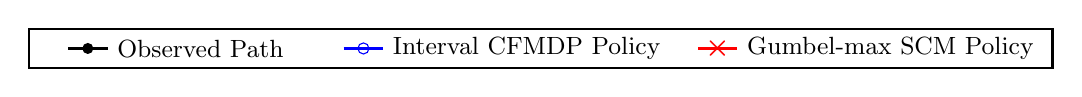
\begin{tikzpicture}[scale=1.0, every node/.style={scale=1.0}]
            \draw[thick, black] (-3, -0.25) rectangle (10, 0.25);
            %
            \draw[black, line width=1pt] (-2.5, 0.0) -- (-2,0.0);
            \fill[black] (-2.25,0.0) circle (2pt); %
            \node[right] at (-2,0.0) {\small Observed Path};
            
            %
            \draw[blue, line width=1pt] (1.0,0.0) -- (1.5,0.0);
            \node[draw=blue, circle, minimum size=4pt, inner sep=0pt] at (1.25,0.0) {}; %
            \node[right] at (1.5,0.0) {\small Interval CFMDP Policy};
            
            %
            \draw[red, line width=1pt] (5.5,0) -- (6,0);
            \node[red] at (5.75,0) {$\boldsymbol{\times}$}; %
            \node[right] at (6,0) {\small Gumbel-max SCM Policy};
        \end{tikzpicture}
    }\\
    %
    \subfigure[\footnotesize Lowest cumulative reward: Interval CFMDP ($312$), Gumbel-max SCM ($312$)]{%
        \resizebox{0.76\columnwidth}{!}{
             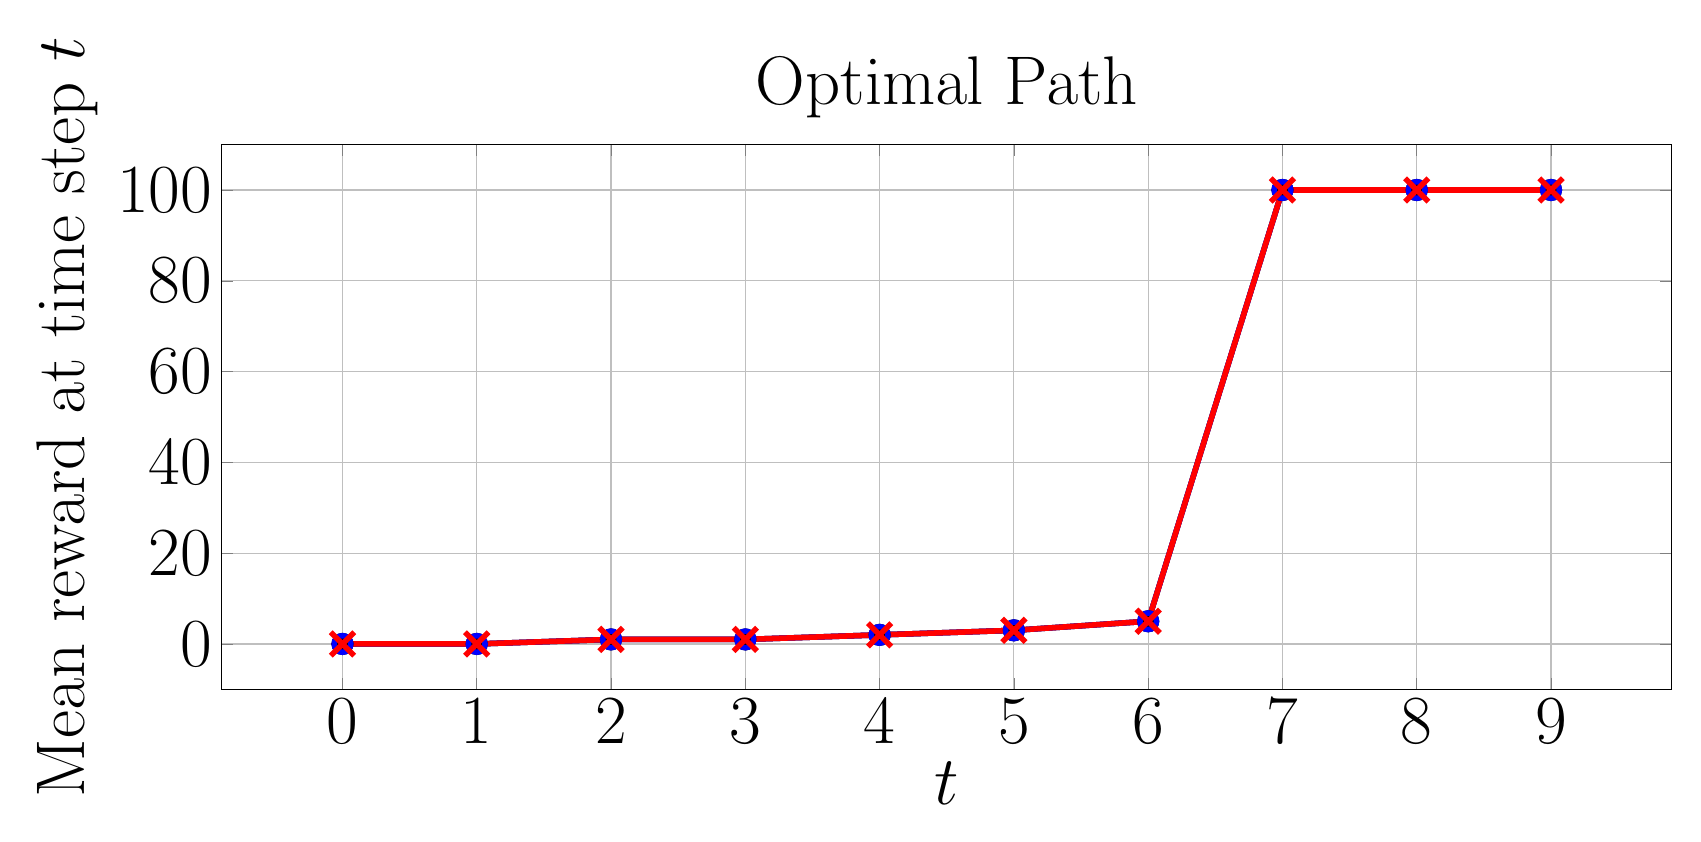
\begin{tikzpicture}
                \begin{axis}[
                    xlabel={$t$},
                    ylabel={Mean reward at time step $t$},
                    title={Optimal Path},
                    grid=both,
                    width=20cm, height=8.5cm,
                    every axis/.style={font=\Huge},
                    %
                ]
                \addplot[
                    color=black, %
                    mark=*, %
                    line width=2pt,
                    mark size=3pt,
                    error bars/.cd,
                    y dir=both, %
                    y explicit, %
                    error bar style={line width=1pt,solid},
                    error mark options={line width=1pt,mark size=4pt,rotate=90}
                ]
                coordinates {
                    (0, 0.0)  +- (0, 0.0)
                    (1, 0.0)  +- (0, 0.0) 
                    (2, 1.0)  +- (0, 0.0) 
                    (3, 1.0)  +- (0, 0.0)
                    (4, 2.0)  +- (0, 0.0)
                    (5, 3.0) +- (0, 0.0)
                    (6, 5.0) +- (0, 0.0)
                    (7, 100.0) +- (0, 0.0)
                    (8, 100.0) +- (0, 0.0)
                    (9, 100.0) +- (0, 0.0)
                };
                %
                \addplot[
                    color=blue, %
                    mark=o, %
                    line width=2pt,
                    mark size=3pt,
                    error bars/.cd,
                    y dir=both, %
                    y explicit, %
                    error bar style={line width=1pt,solid},
                    error mark options={line width=1pt,mark size=4pt,rotate=90}
                ]
                 coordinates {
                    (0, 0.0)  +- (0, 0.0)
                    (1, 0.0)  +- (0, 0.0) 
                    (2, 1.0)  +- (0, 0.0) 
                    (3, 1.0)  +- (0, 0.0)
                    (4, 2.0)  +- (0, 0.0)
                    (5, 3.0) +- (0, 0.0)
                    (6, 5.0) +- (0, 0.0)
                    (7, 100.0) +- (0, 0.0)
                    (8, 100.0) +- (0, 0.0)
                    (9, 100.0) +- (0, 0.0)
                };
                %
                \addplot[
                    color=red, %
                    mark=x, %
                    line width=2pt,
                    mark size=6pt,
                    error bars/.cd,
                    y dir=both, %
                    y explicit, %
                    error bar style={line width=1pt,solid},
                    error mark options={line width=1pt,mark size=4pt,rotate=90}
                ]
                coordinates {
                    (0, 0.0)  +- (0, 0.0)
                    (1, 0.0)  +- (0, 0.0) 
                    (2, 1.0)  +- (0, 0.0) 
                    (3, 1.0)  +- (0, 0.0)
                    (4, 2.0)  +- (0, 0.0)
                    (5, 3.0) +- (0, 0.0)
                    (6, 5.0) +- (0, 0.0)
                    (7, 100.0) +- (0, 0.0)
                    (8, 100.0) +- (0, 0.0)
                    (9, 100.0) +- (0, 0.0)
                };
                \end{axis}
            \end{tikzpicture}
         }
    }
    \hspace{1cm}
    \subfigure[\footnotesize Lowest cumulative reward: Interval CFMDP ($19$), Gumbel-max SCM ($-88$)]{%
         \resizebox{0.76\columnwidth}{!}{
            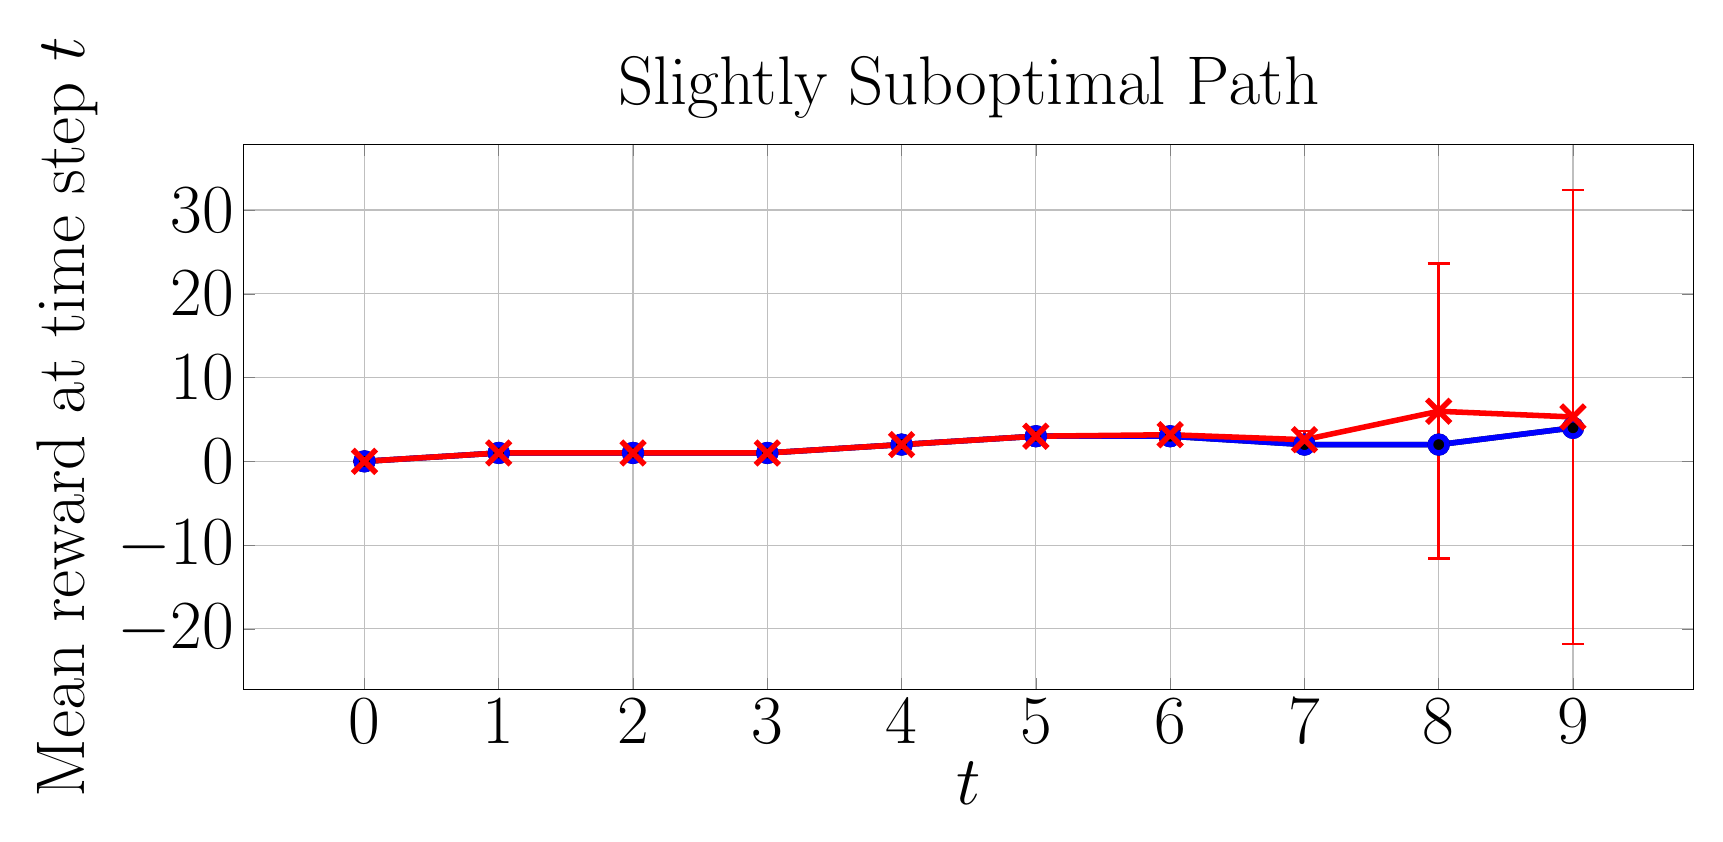
\begin{tikzpicture}
                \begin{axis}[
                    xlabel={$t$},
                    ylabel={Mean reward at time step $t$},
                    title={Slightly Suboptimal Path},
                    grid=both,
                    width=20cm, height=8.5cm,
                    every axis/.style={font=\Huge},
                    %
                ]
                \addplot[
                    color=black, %
                    mark=*, %
                    line width=2pt,
                    mark size=3pt,
                    error bars/.cd,
                    y dir=both, %
                    y explicit, %
                    error bar style={line width=1pt,solid},
                    error mark options={line width=1pt,mark size=4pt,rotate=90}
                ]
              coordinates {
                    (0, 0.0)  +- (0, 0.0)
                    (1, 1.0)  +- (0, 0.0) 
                    (2, 1.0)  +- (0, 0.0) 
                    (3, 1.0)  +- (0, 0.0)
                    (4, 2.0)  +- (0, 0.0)
                    (5, 3.0) +- (0, 0.0)
                    (6, 3.0) +- (0, 0.0)
                    (7, 2.0) +- (0, 0.0)
                    (8, 2.0) +- (0, 0.0)
                    (9, 4.0) +- (0, 0.0)
                };
                %
                \addplot[
                    color=blue, %
                    mark=o, %
                    line width=2pt,
                    mark size=3pt,
                    error bars/.cd,
                    y dir=both, %
                    y explicit, %
                    error bar style={line width=1pt,solid},
                    error mark options={line width=1pt,mark size=4pt,rotate=90}
                ]
              coordinates {
                    (0, 0.0)  +- (0, 0.0)
                    (1, 1.0)  +- (0, 0.0) 
                    (2, 1.0)  +- (0, 0.0) 
                    (3, 1.0)  +- (0, 0.0)
                    (4, 2.0)  +- (0, 0.0)
                    (5, 3.0) +- (0, 0.0)
                    (6, 3.0) +- (0, 0.0)
                    (7, 2.0) +- (0, 0.0)
                    (8, 2.0) +- (0, 0.0)
                    (9, 4.0) +- (0, 0.0)
                };
                %
                \addplot[
                    color=red, %
                    mark=x, %
                    line width=2pt,
                    mark size=6pt,
                    error bars/.cd,
                    y dir=both, %
                    y explicit, %
                    error bar style={line width=1pt,solid},
                    error mark options={line width=1pt,mark size=4pt,rotate=90}
                ]
                coordinates {
                    (0, 0.0)  +- (0, 0.0)
                    (1, 1.0)  +- (0, 0.0) 
                    (2, 1.0)  +- (0, 0.0) 
                    (3, 1.0)  +- (0, 0.0)
                    (4, 2.0)  += (0, 0.0)
                    (5, 3.0)  += (0, 0.0)
                    (6, 3.17847) += (0, 0.62606746) -= (0, 0.62606746)
                    (7, 2.5832885) += (0, 1.04598233) -= (0, 1.04598233)
                    (8, 5.978909) += (0, 17.60137623) -= (0, 17.60137623)
                    (9, 5.297059) += (0, 27.09227512) -= (0, 27.09227512)
                };
                \end{axis}
            \end{tikzpicture}
         }
    }\\[-1.5pt]
    \subfigure[\footnotesize Lowest cumulative reward: Interval CFMDP ($14$), Gumbel-max SCM ($-598$)]{%
         \resizebox{0.76\columnwidth}{!}{
             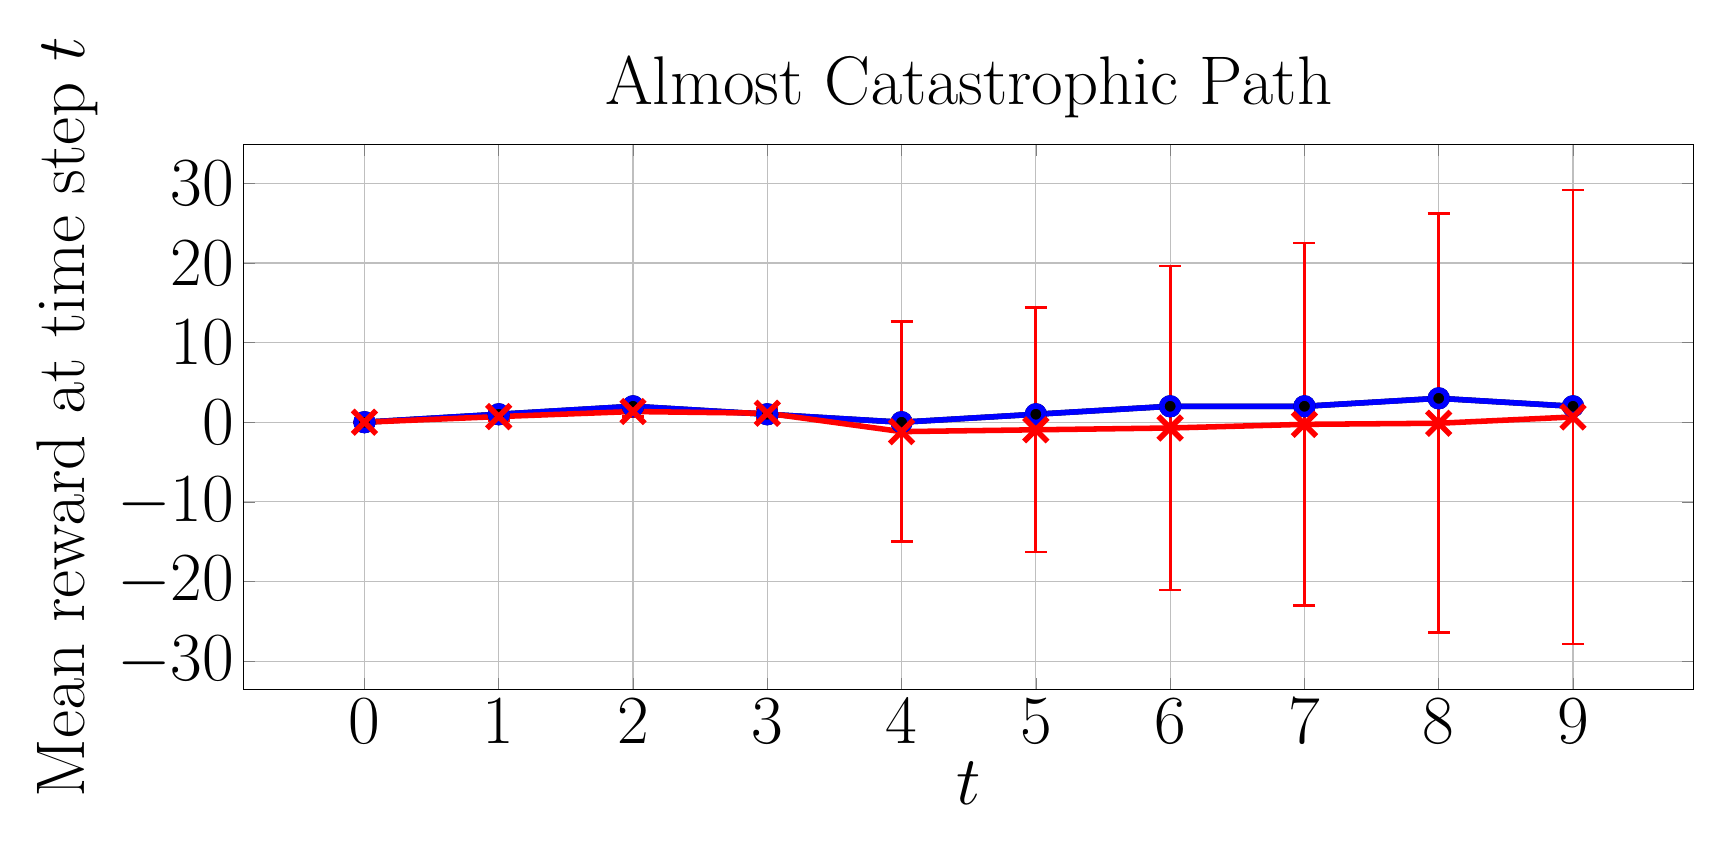
\begin{tikzpicture}
                \begin{axis}[
                    xlabel={$t$},
                    ylabel={Mean reward at time step $t$},
                    title={Almost Catastrophic Path},
                    grid=both,
                    width=20cm, height=8.5cm,
                    every axis/.style={font=\Huge},
                    %
                ]
                \addplot[
                    color=black, %
                    mark=*, %
                    line width=2pt,
                    mark size=3pt,
                    error bars/.cd,
                    y dir=both, %
                    y explicit, %
                    error bar style={line width=1pt,solid},
                    error mark options={line width=1pt,mark size=4pt,rotate=90}
                ]
                coordinates {
                    (0, 0.0)  +- (0, 0.0)
                    (1, 1.0)  +- (0, 0.0) 
                    (2, 2.0)  +- (0, 0.0) 
                    (3, 1.0)  +- (0, 0.0)
                    (4, 0.0)  +- (0, 0.0)
                    (5, 1.0) +- (0, 0.0)
                    (6, 2.0) +- (0, 0.0)
                    (7, 2.0) +- (0, 0.0)
                    (8, 3.0) +- (0, 0.0)
                    (9, 2.0) +- (0, 0.0)
                };
                %
                \addplot[
                    color=blue, %
                    mark=o, %
                    line width=2pt,
                    mark size=3pt,
                    error bars/.cd,
                    y dir=both, %
                    y explicit, %
                    error bar style={line width=1pt,solid},
                    error mark options={line width=1pt,mark size=4pt,rotate=90}
                ]
                coordinates {
                    (0, 0.0)  +- (0, 0.0)
                    (1, 1.0)  +- (0, 0.0) 
                    (2, 2.0)  +- (0, 0.0) 
                    (3, 1.0)  +- (0, 0.0)
                    (4, 0.0)  +- (0, 0.0)
                    (5, 1.0) +- (0, 0.0)
                    (6, 2.0) +- (0, 0.0)
                    (7, 2.0) +- (0, 0.0)
                    (8, 3.0) +- (0, 0.0)
                    (9, 2.0) +- (0, 0.0)
                };
                %
                \addplot[
                    color=red, %
                    mark=x, %
                    line width=2pt,
                    mark size=6pt,
                    error bars/.cd,
                    y dir=both, %
                    y explicit, %
                    error bar style={line width=1pt,solid},
                    error mark options={line width=1pt,mark size=4pt,rotate=90}
                ]
                coordinates {
                    (0, 0.0)  +- (0, 0.0)
                    (1, 0.7065655)  +- (0, 0.4553358) 
                    (2, 1.341673)  +- (0, 0.67091621) 
                    (3, 1.122926)  +- (0, 0.61281824)
                    (4, -1.1821935)  +- (0, 13.82444042)
                    (5, -0.952399)  +- (0, 15.35195457)
                    (6, -0.72672) +- (0, 20.33508414)
                    (7, -0.268983) +- (0, 22.77861454)
                    (8, -0.1310835) +- (0, 26.31013314)
                    (9, 0.65806) +- (0, 28.50670214)
                };
                %
            %
            %
            %
            %
            %
            %
            %
            %
            %
            %
            %
            %
            %
            %
            %
            %
            %
            %
                \end{axis}
            \end{tikzpicture}
         }
    }
    \hspace{1cm}
    \subfigure[\footnotesize Lowest cumulative reward: Interval CFMDP ($-698$), Gumbel-max SCM ($-698$)]{%
         \resizebox{0.76\columnwidth}{!}{
            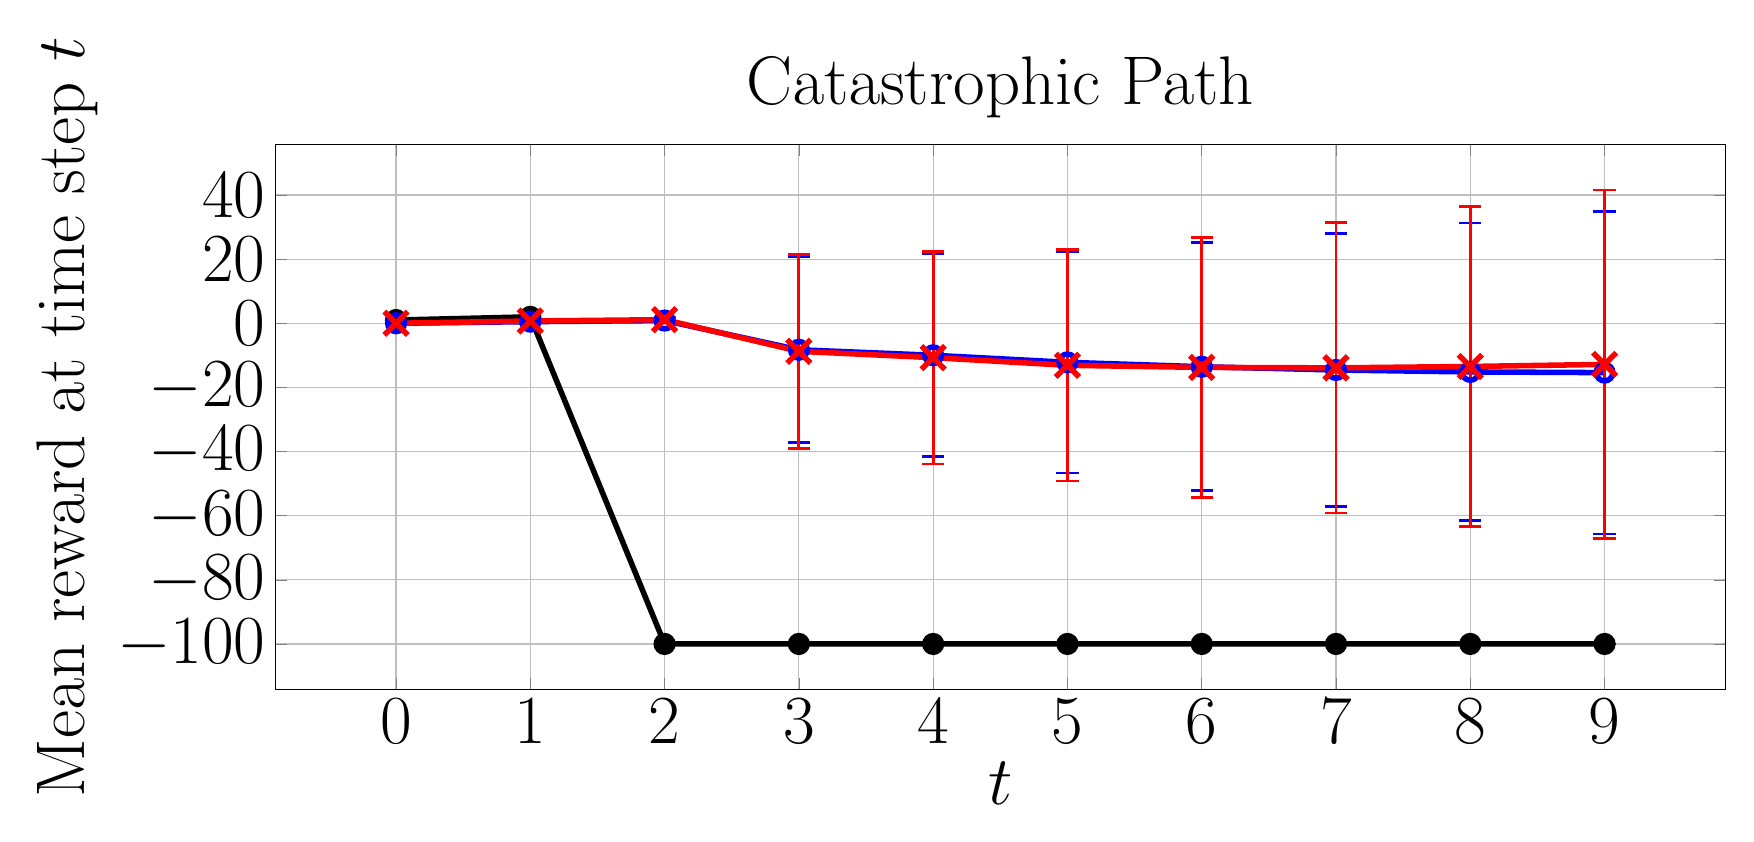
\begin{tikzpicture}
                \begin{axis}[
                    xlabel={$t$},
                    ylabel={Mean reward at time step $t$},
                    title={Catastrophic Path},
                    grid=both,
                    width=20cm, height=8.5cm,
                    every axis/.style={font=\Huge},
                    %
                ]
                \addplot[
                    color=black, %
                    mark=*, %
                    line width=2pt,
                    mark size=3pt,
                    error bars/.cd,
                    y dir=both, %
                    y explicit, %
                    error bar style={line width=1pt,solid},
                    error mark options={line width=1pt,mark size=4pt,rotate=90}
                ]
                coordinates {
                    (0, 1.0)  +- (0, 0.0)
                    (1, 2.0)  +- (0, 0.0) 
                    (2, -100.0)  +- (0, 0.0) 
                    (3, -100.0)  +- (0, 0.0)
                    (4, -100.0)  +- (0, 0.0)
                    (5, -100.0) +- (0, 0.0)
                    (6, -100.0) +- (0, 0.0)
                    (7, -100.0) +- (0, 0.0)
                    (8, -100.0) +- (0, 0.0)
                    (9, -100.0) +- (0, 0.0)
                };
                %
                \addplot[
                    color=blue, %
                    mark=o, %
                    line width=2pt,
                    mark size=3pt,
                    error bars/.cd,
                    y dir=both, %
                    y explicit, %
                    error bar style={line width=1pt,solid},
                    error mark options={line width=1pt,mark size=4pt,rotate=90}
                ]
                coordinates {
                    (0, 0.0)  +- (0, 0.0)
                    (1, 0.504814)  +- (0, 0.49997682) 
                    (2, 0.8439835)  +- (0, 0.76831917) 
                    (3, -8.2709165)  +- (0, 28.93656754)
                    (4, -9.981082)  +- (0, 31.66825363)
                    (5, -12.1776325) +- (0, 34.53463233)
                    (6, -13.556076) +- (0, 38.62845372)
                    (7, -14.574418) +- (0, 42.49603359)
                    (8, -15.1757075) +- (0, 46.41913968)
                    (9, -15.3900395) +- (0, 50.33563368)
                };
                %
                \addplot[
                    color=red, %
                    mark=x, %
                    line width=2pt,
                    mark size=6pt,
                    error bars/.cd,
                    y dir=both, %
                    y explicit, %
                    error bar style={line width=1pt,solid},
                    error mark options={line width=1pt,mark size=4pt,rotate=90}
                ]
                coordinates {
                    (0, 0.0)  +- (0, 0.0)
                    (1, 0.701873)  +- (0, 0.45743556) 
                    (2, 1.1227805)  +- (0, 0.73433129) 
                    (3, -8.7503255)  +- (0, 30.30257976)
                    (4, -10.722092)  +- (0, 33.17618589)
                    (5, -13.10721)  +- (0, 36.0648089)
                    (6, -13.7631645) +- (0, 40.56553451)
                    (7, -13.909043) +- (0, 45.23829402)
                    (8, -13.472517) +- (0, 49.96270296)
                    (9, -12.8278835) +- (0, 54.38618735)
                };
                %
            %
            %
            %
            %
            %
            %
            %
            %
            %
            %
            %
            %
            %
            %
            %
            %
            %
            %
                \end{axis}
            \end{tikzpicture}
         }
    }
    \caption{Average instant reward of CF paths induced by policies on GridWorld $p=0.4$.}
    \label{fig: reward p=0.4}
\end{figure*}

\subsection{Experimental Setup}
To compare policy performance, we measure the average rewards of counterfactual paths induced by our policy and the Gumbel-max policy by uniformly sampling $200$ counterfactual MDPs from the ICFMDP and generating $10,000$ counterfactual paths over each sampled CFMDP. \jl{Since the interval CFMDP depends on the observed path, we select $4$  paths of varying optimality to evaluate how the observed path impacts the performance of both policies: an optimal path, a slightly suboptimal path that could reach the optimal reward with a few changes, a catastrophic path that enters a catastrophic, terminal state with low reward, and an almost catastrophic path that was close to entering a catastrophic state.} When measuring the average probability bound widths and execution time needed to generate the ICFMDPs, we averaged over $20$ randomly generated observed paths
\footnote{Further training details are provided in Appendix \ref{app: training details}, and the code is provided at \href{https://github.com/ddv-lab/robust-cf-inference-in-MDPs}{https://github.com/ddv-lab/robust-cf-inference-in-MDPs}
%
%
.}.

\subsection{GridWorld}
\jl{The GridWorld MDP is a $4 \times 4$ grid where an agent must navigate from the top-left corner to the goal state in the bottom-right corner, avoiding a dangerous terminal state in the centre. At each time step, the agent can move up, down, left, or right, but there is a small probability (controlled by hyper-parameter $p$) of moving in an unintended direction. As the agent nears the goal, the reward for each state increases, culminating in a reward of $+100$ for reaching the goal. Entering the dangerous state results in a penalty of $-100$. We use two versions of GridWorld: a less stochastic version with $p=0.9$ (i.e., $90$\% chance of moving in the chosen direction) and a more stochastic version with $p=0.4$.}

\paragraph{GridWorld ($p=0.9$)}
When $p=0.9$, the counterfactual probability bounds are typically narrow (see Table \ref{tab:nonzero_probs} for average measurements). Consequently, as shown in Figure \ref{fig: reward p=0.9}, both policies are nearly identical and perform similarly well across the optimal, slightly suboptimal, and catastrophic paths.
%
However, for the almost catastrophic path, the interval CFMDP path is more conservative and follows the observed path more closely (as this is where the probability bounds are narrowest), which typically requires one additional step to reach the goal state than the Gumbel-max SCM policy.
%

\paragraph{GridWorld ($p=0.4$)}
\jl{When $p=0.4$, the GridWorld environment becomes more uncertain, increasing the risk of entering the dangerous state even if correct actions are chosen. Thus, as shown in Figure \ref{fig: reward p=0.4}, the interval CFMDP policy adopts a more conservative approach, avoiding deviation from the observed policy if it cannot guarantee higher counterfactual rewards (see the slightly suboptimal and almost catastrophic paths), whereas the Gumbel-max SCM is inconsistent: it can yield higher rewards, but also much lower rewards, reflected in the wide error bars.} For the catastrophic path, both policies must deviate from the observed path to achieve a higher reward and, in this case, perform similarly.
%
%
%
%
\subsection{Sepsis}
The Sepsis MDP \citep{oberst2019counterfactual} simulates trajectories of Sepsis patients. Each state consists of four vital signs (heart rate, blood pressure, oxygen concentration, and glucose levels), categorised as low, normal, or high.
and three treatments that can be toggled on/off at each time step (8 actions in total). Unlike \citet{oberst2019counterfactual}, we scale rewards based on the number of out-of-range vital signs, between $-1000$ (patient dies) and $1000$ (patient discharged). \jl{Like the GridWorld $p=0.4$ experiment, the Sepsis MDP is highly uncertain, as many states are equally likely to lead to optimal and poor outcomes. Thus, as shown in Figure \ref{fig: reward sepsis}, both policies follow the observed optimal and almost catastrophic paths to guarantee rewards are no worse than the observation.} However, improving the catastrophic path requires deviating from the observation. Here, the Gumbel-max SCM policy, on average, performs better than the interval CFMDP policy. But, since both policies have lower bounds clipped at $-1000$, neither policy reliably improves over the observation. In contrast, for the slightly suboptimal path, the interval CFMDP policy performs significantly better, shown by its higher lower bounds. 
Moreover, in these two cases, the worst-case counterfactual path generated by the interval CFMDP policy is better than that of the Gumbel-max SCM policy,
indicating its greater robustness.
%
\begin{figure*}
    \centering
     \resizebox{0.6\textwidth}{!}{
        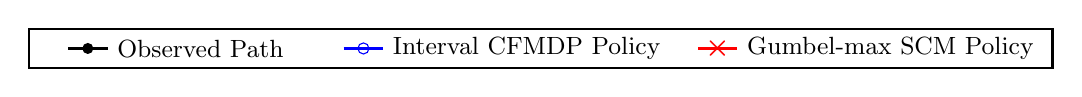
\begin{tikzpicture}[scale=1.0, every node/.style={scale=1.0}]
            \draw[thick, black] (-3, -0.25) rectangle (10, 0.25);
            %
            \draw[black, line width=1pt] (-2.5, 0.0) -- (-2,0.0);
            \fill[black] (-2.25,0.0) circle (2pt); %
            \node[right] at (-2,0.0) {\small Observed Path};
            
            %
            \draw[blue, line width=1pt] (1.0,0.0) -- (1.5,0.0);
            \node[draw=blue, circle, minimum size=4pt, inner sep=0pt] at (1.25,0.0) {}; %
            \node[right] at (1.5,0.0) {\small Interval CFMDP Policy};
            
            %
            \draw[red, line width=1pt] (5.5,0) -- (6,0);
            \node[red] at (5.75,0) {$\boldsymbol{\times}$}; %
            \node[right] at (6,0) {\small Gumbel-max SCM Policy};
        \end{tikzpicture}
    }\\
    \subfigure[\footnotesize Lowest cumulative reward: Interval CFMDP ($8000$), Gumbel-max SCM ($8000$)]{%
         \resizebox{0.76\columnwidth}{!}{
             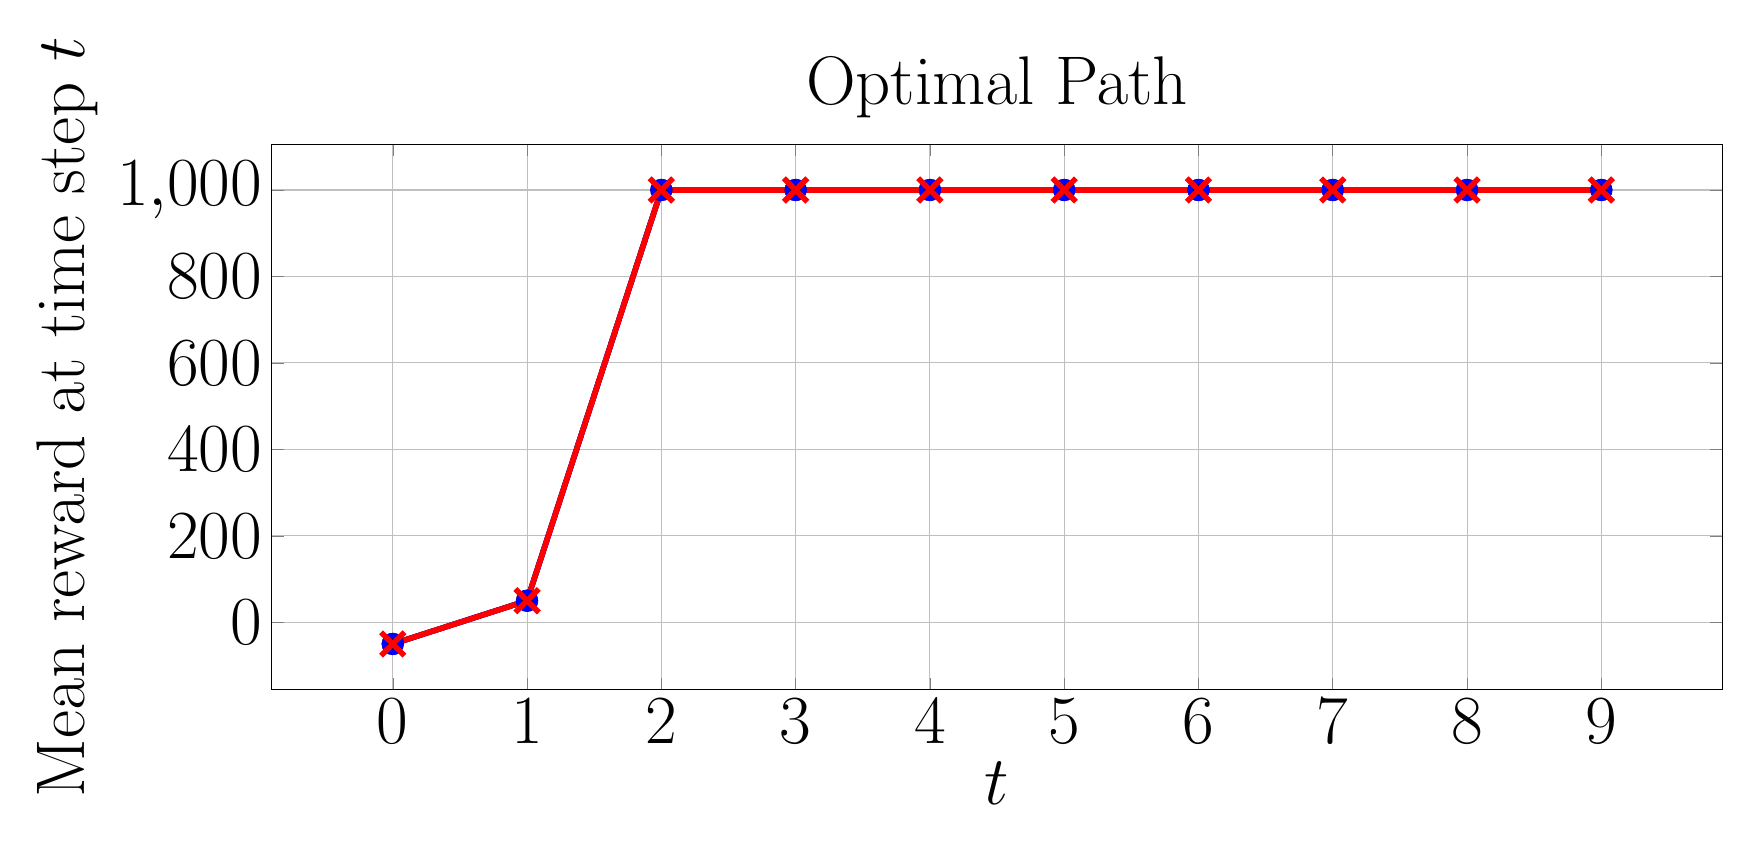
\begin{tikzpicture}
                \begin{axis}[
                    xlabel={$t$},
                    ylabel={Mean reward at time step $t$},
                    title={Optimal Path},
                    grid=both,
                    width=20cm, height=8.5cm,
                    every axis/.style={font=\Huge},
                    %
                ]
                \addplot[
                    color=black, %
                    mark=*, %
                    line width=2pt,
                    mark size=3pt,
                ]
                coordinates {
                    (0, -50.0)
                    (1, 50.0)
                    (2, 1000.0)
                    (3, 1000.0)
                    (4, 1000.0)
                    (5, 1000.0)
                    (6, 1000.0)
                    (7, 1000.0)
                    (8, 1000.0)
                    (9, 1000.0)
                };
                %
                \addplot[
                    color=blue, %
                    mark=o, %
                    line width=2pt,
                    mark size=3pt,
                    error bars/.cd,
                    y dir=both, %
                    y explicit, %
                    error bar style={line width=1pt,solid},
                    error mark options={line width=1pt,mark size=4pt,rotate=90}
                ]
                coordinates {
                    (0, -50.0)  +- (0, 0.0)
                    (1, 50.0)  +- (0, 0.0) 
                    (2, 1000.0)  +- (0, 0.0) 
                    (3, 1000.0)  +- (0, 0.0)
                    (4, 1000.0)  +- (0, 0.0)
                    (5, 1000.0) +- (0, 0.0)
                    (6, 1000.0) +- (0, 0.0)
                    (7, 1000.0) +- (0, 0.0)
                    (8, 1000.0) +- (0, 0.0)
                    (9, 1000.0) +- (0, 0.0)
                };
                %
                \addplot[
                    color=red, %
                    mark=x, %
                    line width=2pt,
                    mark size=6pt,
                    error bars/.cd,
                    y dir=both, %
                    y explicit, %
                    error bar style={line width=1pt,solid},
                    error mark options={line width=1pt,mark size=4pt,rotate=90}
                ]
                coordinates {
                    (0, -50.0)  +- (0, 0.0)
                    (1, 50.0)  +- (0, 0.0) 
                    (2, 1000.0)  +- (0, 0.0) 
                    (3, 1000.0)  +- (0, 0.0)
                    (4, 1000.0)  +- (0, 0.0)
                    (5, 1000.0) +- (0, 0.0)
                    (6, 1000.0) +- (0, 0.0)
                    (7, 1000.0) +- (0, 0.0)
                    (8, 1000.0) +- (0, 0.0)
                    (9, 1000.0) +- (0, 0.0)
                };
                %
                \end{axis}
            \end{tikzpicture}
         }
    }
    \hspace{1cm}
    \subfigure[\footnotesize Lowest cumulative reward: Interval CFMDP ($-5980$), Gumbel-max SCM ($-8000$)]{%
         \resizebox{0.76\columnwidth}{!}{
            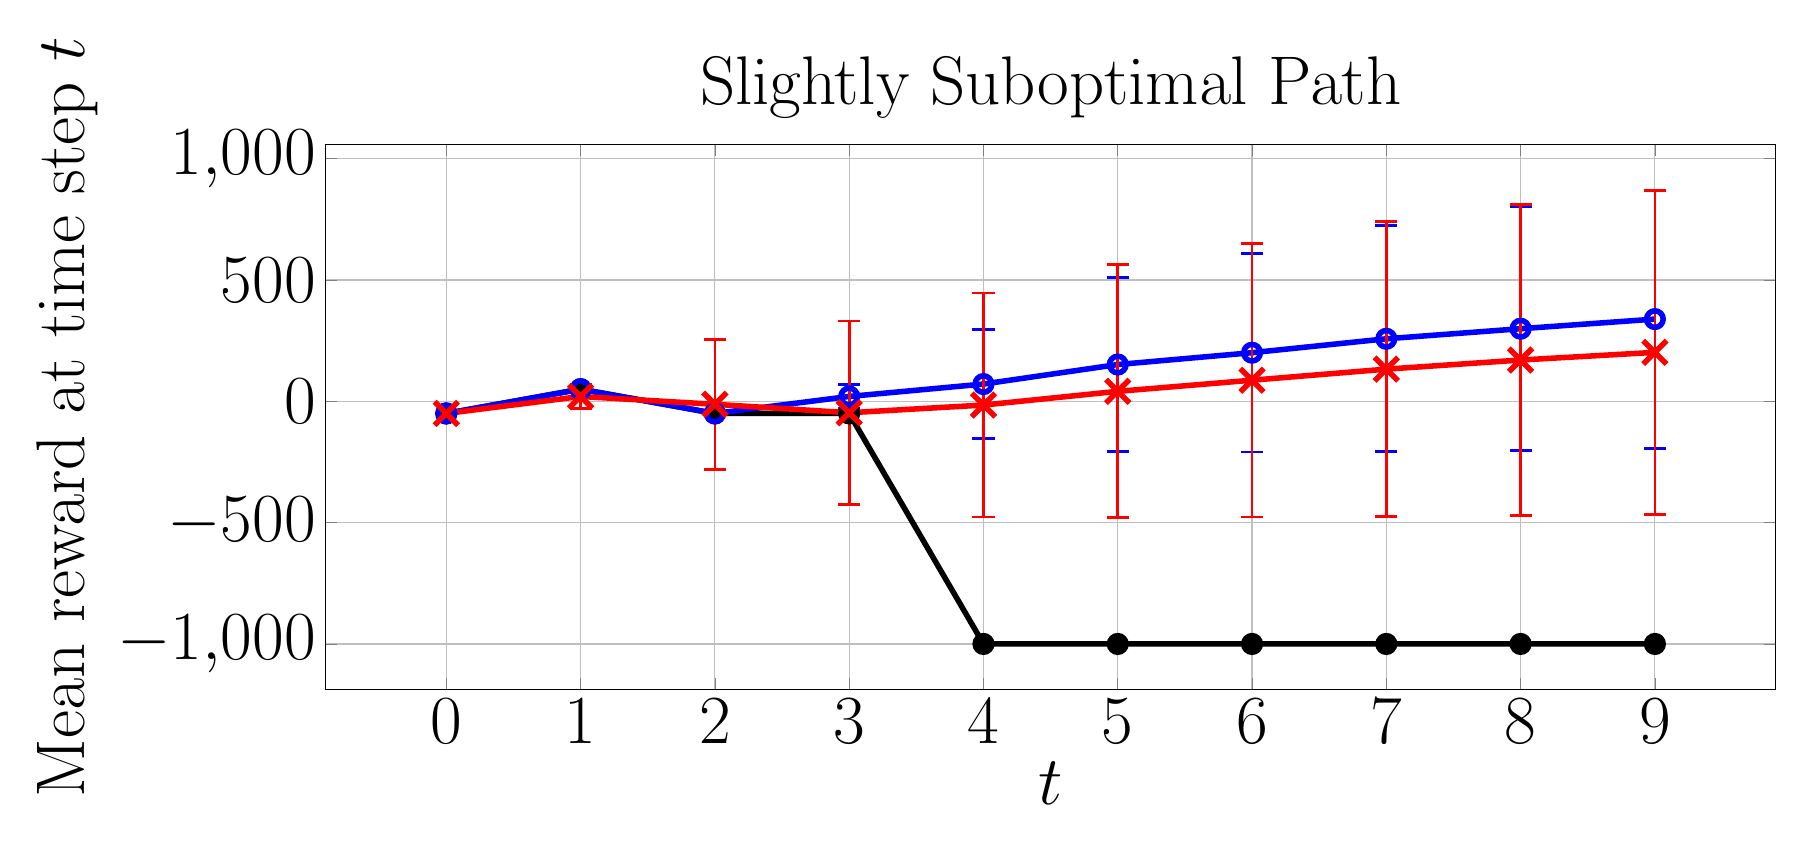
\begin{tikzpicture}
                \begin{axis}[
                    xlabel={$t$},
                    ylabel={Mean reward at time step $t$},
                    title={Slightly Suboptimal Path},
                    grid=both,
                    width=20cm, height=8.5cm,
                    every axis/.style={font=\Huge},
                    %
                ]
               \addplot[
                    color=black, %
                    mark=*, %
                    line width=2pt,
                    mark size=3pt,
                ]
                coordinates {
                    (0, -50.0)
                    (1, 50.0)
                    (2, -50.0)
                    (3, -50.0)
                    (4, -1000.0)
                    (5, -1000.0)
                    (6, -1000.0)
                    (7, -1000.0)
                    (8, -1000.0)
                    (9, -1000.0)
                };
                %
                \addplot[
                    color=blue, %
                    mark=o, %
                    line width=2pt,
                    mark size=3pt,
                    error bars/.cd,
                    y dir=both, %
                    y explicit, %
                    error bar style={line width=1pt,solid},
                    error mark options={line width=1pt,mark size=4pt,rotate=90}
                ]
                coordinates {
                    (0, -50.0)  +- (0, 0.0)
                    (1, 50.0)  +- (0, 0.0) 
                    (2, -50.0)  +- (0, 0.0) 
                    (3, 20.0631)  +- (0, 49.97539413)
                    (4, 71.206585)  +- (0, 226.02033693)
                    (5, 151.60797) +- (0, 359.23292559)
                    (6, 200.40593) +- (0, 408.86185176)
                    (7, 257.77948) +- (0, 466.10372804)
                    (8, 299.237465) +- (0, 501.82579506)
                    (9, 338.9129) +- (0, 532.06124996)
                };
                %
                \addplot[
                    color=red, %
                    mark=x, %
                    line width=2pt,
                    mark size=6pt,
                    error bars/.cd,
                    y dir=both, %
                    y explicit, %
                    error bar style={line width=1pt,solid},
                    error mark options={line width=1pt,mark size=4pt,rotate=90}
                ]
                coordinates {
                    (0, -50.0)  +- (0, 0.0)
                    (1, 20.00736)  +- (0, 49.99786741) 
                    (2, -12.282865)  +- (0, 267.598755) 
                    (3, -47.125995)  +- (0, 378.41755832)
                    (4, -15.381965)  +- (0, 461.77616558)
                    (5, 41.15459) +- (0, 521.53189262)
                    (6, 87.01595) +- (0, 564.22243126 )
                    (7, 132.62376) +- (0, 607.31338037)
                    (8, 170.168145) +- (0, 641.48013693)
                    (9, 201.813135) +- (0, 667.29441777)
                };
                %
                %
                %
                %
                %
                %
                %
                %
                %
                %
                %
                %
                %
                %
                %
                %
                %
                %
                %
                \end{axis}
            \end{tikzpicture}
         }
    }\\[-1.5pt]
    \subfigure[\footnotesize Lowest cumulative reward: Interval CFMDP ($100$), Gumbel-max SCM ($100$)]{%
         \resizebox{0.76\columnwidth}{!}{
             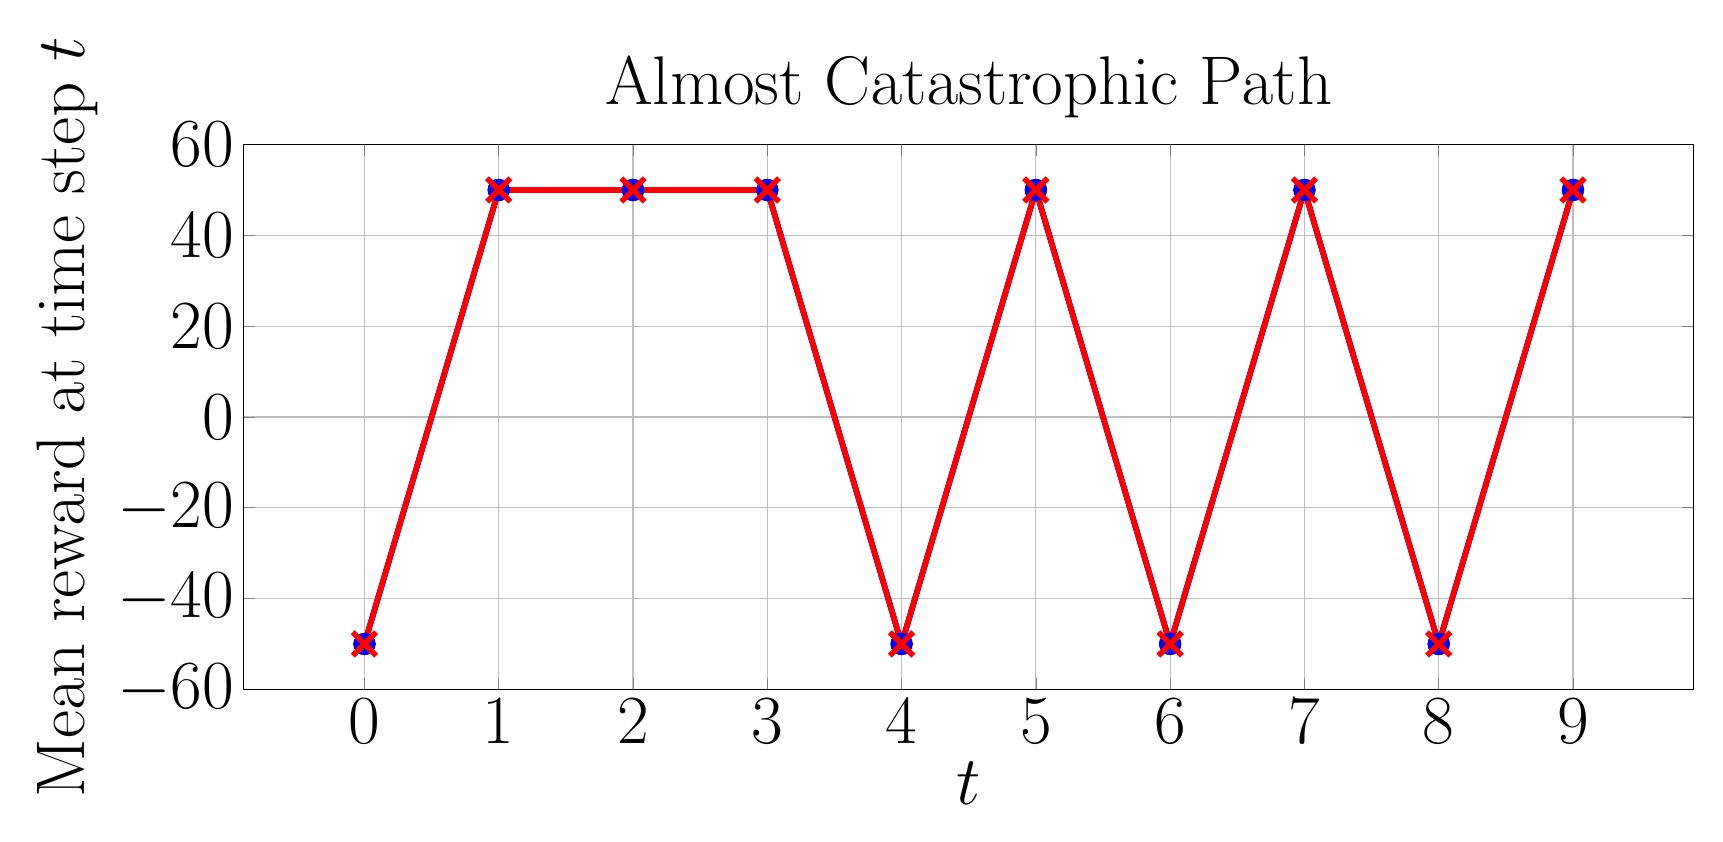
\begin{tikzpicture}
                \begin{axis}[
                    xlabel={$t$},
                    ylabel={Mean reward at time step $t$},
                    title={Almost Catastrophic Path},
                    grid=both,
                    every axis/.style={font=\Huge},
                    width=20cm, height=8.5cm,
                    %
                ]
               \addplot[
                    color=black, %
                    mark=*, %
                    line width=2pt,
                    mark size=3pt,
                ]
                coordinates {
                    (0, -50.0)
                    (1, 50.0)
                    (2, 50.0)
                    (3, 50.0)
                    (4, -50.0)
                    (5, 50.0)
                    (6, -50.0)
                    (7, 50.0)
                    (8, -50.0)
                    (9, 50.0)
                };
                %
                %
                \addplot[
                    color=blue, %
                    mark=o, %
                    line width=2pt,
                    mark size=3pt,
                    error bars/.cd,
                    y dir=both, %
                    y explicit, %
                    error bar style={line width=1pt,solid},
                    error mark options={line width=1pt,mark size=4pt,rotate=90}
                ]
                coordinates {
                    (0, -50.0)  +- (0, 0.0)
                    (1, 50.0)  +- (0, 0.0) 
                    (2, 50.0)  +- (0, 0.0) 
                    (3, 50.0)  +- (0, 0.0)
                    (4, -50.0)  +- (0, 0.0)
                    (5, 50.0) +- (0, 0.0)
                    (6, -50.0) +- (0, 0.0)
                    (7, 50.0) +- (0, 0.0)
                    (8, -50.0) +- (0, 0.0)
                    (9, 50.0) +- (0, 0.0)
                };
                %
                \addplot[
                    color=red, %
                    mark=x, %
                    line width=2pt,
                    mark size=6pt,
                    error bars/.cd,
                    y dir=both, %
                    y explicit, %
                    error bar style={line width=1pt,solid},
                    error mark options={line width=1pt,mark size=4pt,rotate=90}
                ]
                coordinates {
                    (0, -50.0)  +- (0, 0.0)
                    (1, 50.0)  +- (0, 0.0) 
                    (2, 50.0)  +- (0, 0.0) 
                    (3, 50.0)  +- (0, 0.0)
                    (4, -50.0)  +- (0, 0.0)
                    (5, 50.0) +- (0, 0.0)
                    (6, -50.0) +- (0, 0.0)
                    (7, 50.0) +- (0, 0.0)
                    (8, -50.0) +- (0, 0.0)
                    (9, 50.0) +- (0, 0.0)
                };
                %
                %
                %
                %
                %
                %
                %
                %
                %
                %
                %
                %
                %
                %
                %
                %
                %
                %
                %
                \end{axis}
            \end{tikzpicture}
         }
    }
    \hspace{1cm}
    \subfigure[\footnotesize Lowest cumulative reward: Interval CFMDP ($-7150$), Gumbel-max SCM ($-9050$)]{%
         \resizebox{0.76\columnwidth}{!}{
            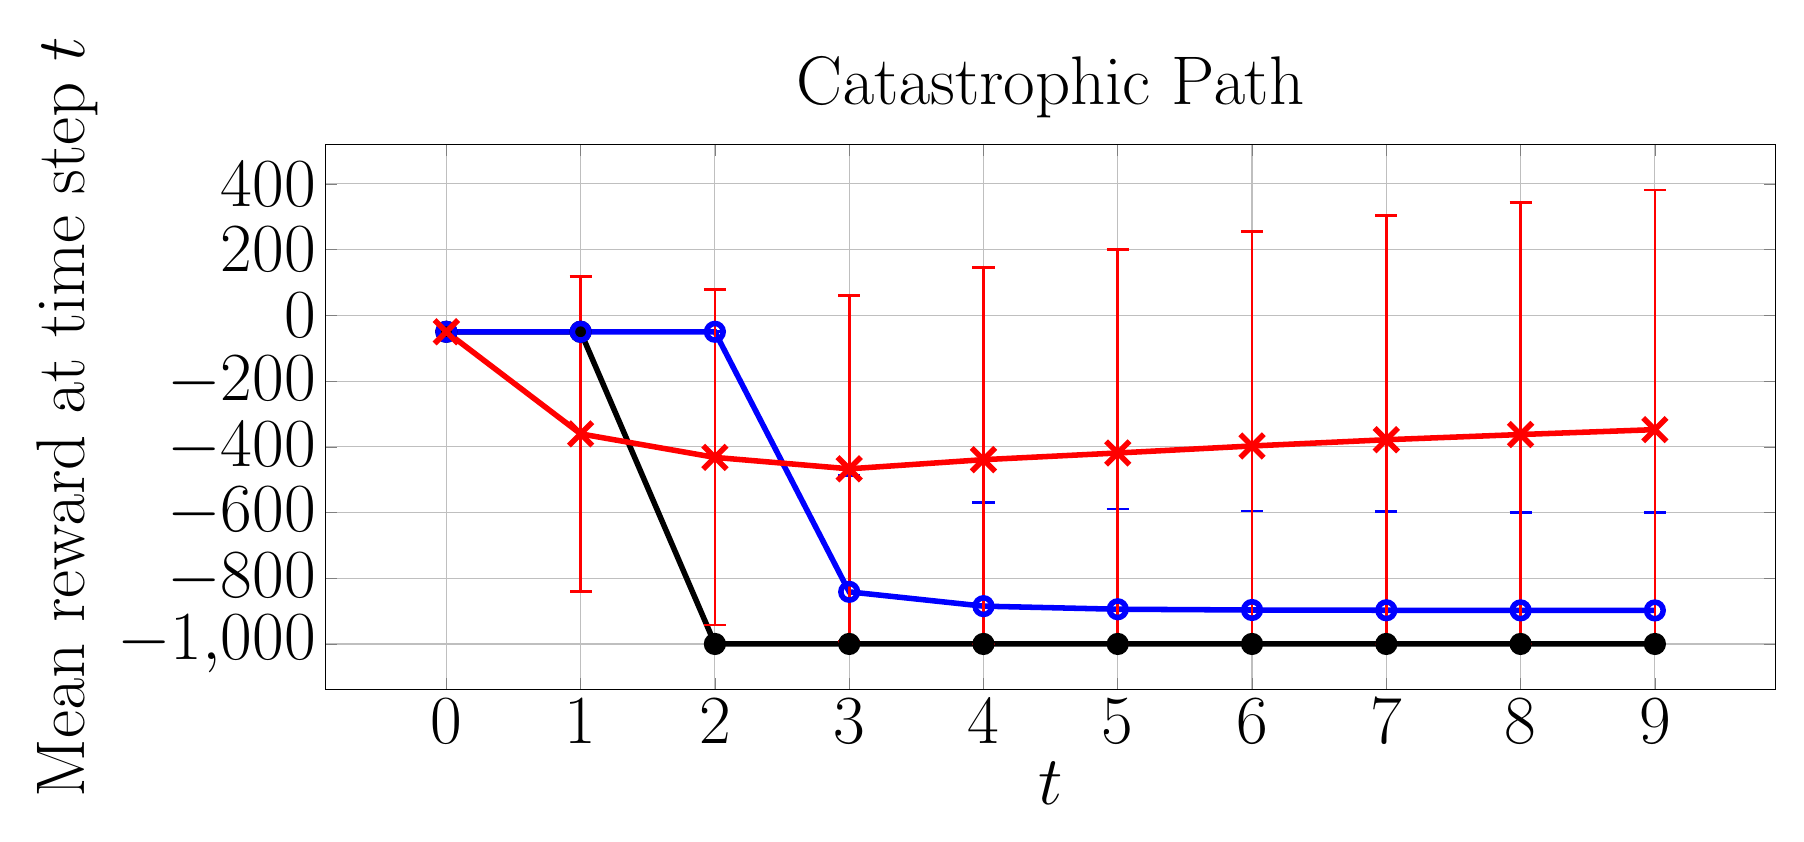
\begin{tikzpicture}
                \begin{axis}[
                    xlabel={$t$},
                    ylabel={Mean reward at time step $t$},
                    title={Catastrophic Path},
                    grid=both,
                    width=20cm, height=8.5cm,
                    every axis/.style={font=\Huge},
                    %
                ]
               \addplot[
                    color=black, %
                    mark=*, %
                    line width=2pt,
                    mark size=3pt,
                ]
                coordinates {
                    (0, -50.0)
                    (1, -50.0)
                    (2, -1000.0)
                    (3, -1000.0)
                    (4, -1000.0)
                    (5, -1000.0)
                    (6, -1000.0)
                    (7, -1000.0)
                    (8, -1000.0)
                    (9, -1000.0)
                };
                %
                %
                \addplot[
                    color=blue, %
                    mark=o, %
                    line width=2pt,
                    mark size=3pt,
                    error bars/.cd,
                    y dir=both, %
                    y explicit, %
                    error bar style={line width=1pt,solid},
                    error mark options={line width=1pt,mark size=4pt,rotate=90}
                ]
                coordinates {
                    (0, -50.0)  +- (0, 0.0)
                    (1, -50.0)  +- (0, 0.0) 
                    (2, -50.0)  +- (0, 0.0) 
                    (3, -841.440725)  += (0, 354.24605512) -= (0, 158.559275)
                    (4, -884.98225)  += (0, 315.37519669) -= (0, 115.01775)
                    (5, -894.330425) += (0, 304.88572805) -= (0, 105.669575)
                    (6, -896.696175) += (0, 301.19954514) -= (0, 103.303825)
                    (7, -897.4635) += (0, 299.61791279) -= (0, 102.5365)
                    (8, -897.77595) += (0, 298.80392585) -= (0, 102.22405)
                    (9, -897.942975) += (0, 298.32920557) -= (0, 102.057025)
                };
                %
                \addplot[
                    color=red, %
                    mark=x, %
                    line width=2pt,
                    mark size=6pt,
                    error bars/.cd,
                    y dir=both, %
                    y explicit, %
                    error bar style={line width=1pt,solid},
                    error mark options={line width=1pt,mark size=4pt,rotate=90}
                ]
            coordinates {
                    (0, -50.0)  +- (0, 0.0)
                    (1, -360.675265)  +- (0, 479.39812699) 
                    (2, -432.27629)  +- (0, 510.38620897) 
                    (3, -467.029545)  += (0, 526.36009628) -= (0, 526.36009628)
                    (4, -439.17429)  += (0, 583.96638919) -= (0, 560.82571)
                    (5, -418.82704) += (0, 618.43027478) -= (0, 581.17296)
                    (6, -397.464895) += (0, 652.67322574) -= (0, 602.535105)
                    (7, -378.49052) += (0, 682.85407033) -= (0, 621.50948)
                    (8, -362.654195) += (0, 707.01412023) -= (0, 637.345805)
                    (9, -347.737935) += (0, 729.29076479) -= (0, 652.262065)
                };
                %
                %
                %
                %
                %
                %
                %
                %
                %
                %
                %
                %
                %
                %
                %
                %
                %
                %
                %
                \end{axis}
            \end{tikzpicture}
         }
    }
    \caption{Average instant reward of CF paths induced by policies on Sepsis.}
    \label{fig: reward sepsis}
\end{figure*}

%
%
%
\subsection{Interval CFMDP Bounds}
%
%
Table \ref{tab:nonzero_probs} presents the mean counterfactual probability bound widths (excluding transitions where the upper bound is $0$) for each MDP, averaged over 20 observed paths. We compare the bounds under counterfactual stability (CS) and monotonicity (M) assumptions, CS alone, and no assumptions. This shows that the assumptions marginally reduce the bound widths, indicating the assumptions tighten the bounds without excluding too many causal models, as intended.
\renewcommand{\arraystretch}{1}

\begin{table}
\centering
\caption{Mean width of counterfactual probability bounds}
\resizebox{0.8\columnwidth}{!}{%
\begin{tabular}{|c|c|c|c|}
\hline
\multirow{2}{*}{\textbf{Environment}} & \multicolumn{3}{c|}{\textbf{Assumptions}} \\ \cline{2-4}
 & \textbf{CS + M} & \textbf{CS} & \textbf{None\tablefootnote{\jl{Equivalent to \citet{li2024probabilities}'s bounds (see Section \ref{sec: equivalence with Li}).}}} \\ \hline
\textbf{GridWorld} ($p=0.9$) & 0.0817 & 0.0977 & 0.100 \\ \hline
\textbf{GridWorld} ($p=0.4$) & 0.552  & 0.638  & 0.646 \\ \hline
\textbf{Sepsis} & 0.138 & 0.140 & 0.140 \\ \hline
\end{tabular}
}
\label{tab:nonzero_probs}
\end{table}


\subsection{Execution Times}
Table \ref{tab: times} compares the average time needed to generate the interval CFMDP vs.\ the Gumbel-max SCM CFMDP for 20 observations.
The GridWorld algorithms were run single-threaded, while the Sepsis experiments were run in parallel.
Generating the interval CFMDP is significantly faster as it uses exact analytical bounds, whereas the Gumbel-max CFMDP requires sampling from the Gumbel distribution to estimate counterfactual transition probabilities. \jl{Since constructing the counterfactual MDP models is the main bottleneck in both approaches, ours is more efficient overall and suitable for larger MDPs.}
\begin{table}
\centering
\caption{Mean execution time to generate CFMDPs}
\resizebox{0.99\columnwidth}{!}{%
\begin{tabular}{|c|c|c|}
\hline
\multirow{2}{*}{\textbf{Environment}} & \multicolumn{2}{c|}{\textbf{Mean Execution Time (s)}} \\ \cline{2-3} 
                                      & \textbf{Interval CFMDP} & \textbf{Gumbel-max CFMDP} \\ \hline
\textbf{GridWorld ($p=0.9$) }                  & 0.261                   & 56.1                      \\ \hline
\textbf{GridWorld ($p=0.4$)  }                 & 0.336                   & 54.5                      \\ \hline
\textbf{Sepsis}                                 & 688                     & 2940                      \\ \hline
\end{tabular}%
}
\label{tab: times}
\end{table}

\section{Results}





\subsection{Evaluation of generated images} \label{subsection: Evaluation of generated images}

%The generative capabilities of the model are evaluated with quantitative metrics and with a visual Turing test. 
%To fairly evaluate the generated images directly to the reference CAMUS images, the evaluation experiments in this subsection do not use the sector width augmentations explained in subsection \ref{subsection: Training of the DDPM}. These additional augmentations do not affect the metrics by a lot, but would \newline


The ImageNet Fréchet inception distance (FID) \cite{heusel2017gans} and inception score (IS) \cite{salimans2016improved}
of the diffusion model are 23.87 and 1.47 respectively. However, these metrics can give misleading results for generative models that are not trained on ImageNet \cite{deng2009imagenet, barratt2018note, rosca2017variational}. To qualitatively assess the performance of the model, Fig.~\ref{fig: similar_samples} shows random samples generated together with the most similar cases from the CAMUS dataset identified automatically using the structural similarity index measure (SSIM) \cite{wang2004image}. This shows the model does not simply memorize cases from the training set, and produces realistic and varied samples. \newline




\begin{figure*}[h]
\centering
  \centering
  \includegraphics[trim={0.75cm 0.25cm 0.75cm 0.25cm}, clip,width = 1\linewidth]{figures/similar_samples_v2.drawio.pdf}
  \caption{Generated samples, together with most similar cases in the train and validation set and the test set of the CAMUS dataset, based on SSIM \cite{wang2004image}.}
  \label{fig: similar_samples}
\end{figure*}

\subsection{Survey results}

On the 45 pairs with one real and one synthetic image, participants correctly identified the synthetic image 56.4\% of the time. When broken down by group, cardiologists achieved an accuracy of 63.7\%, while clinical researchers and engineers both identified the correct frame 53.3\% of the time. Fig.~\ref{fig: survey} shows the explanations given when the participants correctly identified the synthetic frame, when they were wrong, and when both frames were real in the 5 cases mentioned above.
\newline

Using a binomial test with a significance level of 5\%, the accuracy of the cardiologists was found to be statistically significantly higher than random guessing ($P=0.09\%$). However, the engineers and clinical researchers in the survey did not show statistically significant higher accuracy compared to random guessing ($P=24.6\%$).

\begin{figure*}[h]
\centering
  \centering
  \includegraphics[trim={0cm 0cm 0cm 0cm}, clip,width = 1\linewidth]{figures/combined_reasons_grouped_barplot.pdf}
  \caption{Explanations given during the survey}
  \label{fig: survey}
\end{figure*}





%In the visual Turing test experiment, two ultrasound engineers and one clinician were shown an image and asked to determine whether it was real or synthetic. The images consisted of 50 frames sampled randomly from the CAMUS dataset and 50 frames sampled from the DDPM trained on the CAMUS dataset. These 100 images were presented to the respondents in a random order. If the respondents identified a frame as synthetic, they had to select a reason from the pre-defined options "Anatomically incorrect," "Speckle patterns," or "Image artifacts." If none of these options matched their reasoning, they could select "Other" and provide an explanation in a text field. Figure \ref{fig: survey} shows the results of the survey.

%\begin{figure}
%     \centering
%     \begin{subfigure}[b]{0.8\linewidth}
%         \centering \includegraphics[trim={0.2cm 0.2cm 0.2cm 0.2cm}, clip, width=1\linewidth]{figures/survey_results.pdf}
%         \caption{Results of the visual Turing test.}
%     \end{subfigure}
%     \begin{subfigure}[b]{0.8\linewidth}
%         \centering \includegraphics[trim={0.2cm 0.2cm 0.2cm 0.2cm}, clip, width=1\linewidth]{figures/survey_reasons.pdf}\caption{Explanations given for selecting synthetic}
%         \label{fig: survey_reasons}
%     \end{subfigure}
%   \caption{Results of the visual Turing test survey. For each image labeled as synthetic, the respondents where asked to indicate a reason for selecting synthetic.}
%    \label{fig: survey}
%\end{figure}

\subsection{Segmentation ablation study results}

Table \ref{table: ablation_study_1} shows the results of the ablation study on the CAMUS dataset, using Dice score and Hausdorff distance as metrics. The bottom part of Fig.~\ref{fig: heatmaps} shows the heatmaps of pixels belonging to the LV after applying the combination of all generative augmentations. Comparing these to the original illustrates that the generative augmentations increase the variety of LV location in the image. \newline

The increase in segmentation accuracy of the HUNT4 model on CAMUS originate mostly from an improvement in segmentation accuracy for samples outside the HUNT4 image distribution. Table \ref{table: camus_subsets_results} lists the segmentation results for the HUNT4 models on different subsets of CAMUS. The subsets are based on depth and sector angle cutoff values visualized in Figs.~\ref{fig: depths_hist} and \ref{fig: sector_angles_hist}.


%Subsection \ref{subsection: results of segmentation ablation study} contains the result of the ablation study. 



\begin{table*}[h]
\scriptsize
  \centering
  \renewcommand{\arraystretch}{1} % Increase vertical spacing
  \caption{Segmentation results of the ablation study using different datasets (HUNT4 and CAMUS) for training and testing. For all experiments, regular augmentations are applied in addition to the generative augmentations (see Table \ref{table: characteristics nnunet}).The Dice score and Hausdorff distance are only for the LV lumen label. We elaborate on this choice in the Discussion. Since the two datasets have been annotated by different experts with different annotation conventions, there is a considerably lower segmentation accuracy when the training and test sets are different. }
  \begin{tabular}{m{60pt}m{40pt}m{120pt}m{60pt}m{100pt}}
    \toprule
      Training set  & Test set & Generative Augmentations & Dice score & Hausdorff distance (mm)\\
    \midrule
    \multirow{7}{1.4cm}{HUNT4} & \multirow{7}{1.4cm}{CAMUS} & None & 0.802 $\pm$ 0.15 & 29.03 $\pm$ 26.01\\
    && Depth increase & 0.887 $\pm$ 0.05 & \textbf{7.49 $\pm$ 3.25} \\
    && Tilt variation  & 0.829 $\pm$ 0.14 & 17.31 $\pm$ 20.98 \\
    && Sector width & 0.847 $\pm$ 0.11 & 21.36 $\pm$ 23.84\\
    && Translation & 0.840 $\pm$ 0.12 & 16.55 $\pm$ 19.71 \\
    && Combination & \textbf{0.887 $\pm$ 0.05} & 8.17 $\pm$ 5.32 \\
    && Combination without repaint & 0.810 $\pm$ 0.15  & 26.90 $\pm$ 25.07\\
    \midrule
    \multirow{7}{1.4cm}{CAMUS} &  \multirow{7}{1.4cm}{CAMUS} & None & 0.943 $\pm$ 0.03 & 4.46 $\pm$ 2.52 \\
    && Depth increase & 0.945 $\pm$ 0.03 & \textbf{4.27 $\pm$ 2.34} \\
    && Tilt variation  &  0.945 $\pm$ 0.03 &  4.30 $\pm$ 2.43 \\
    && Sector width variation & \textbf{0.946 $\pm$ 0.03} & 4.34 $\pm$ 2.41 \\
    && Translation & 0.944 $\pm$ 0.03 & 4.44 $\pm$ 2.43\\
    && Combination & 0.944 $\pm$ 0.03 & 4.37 $\pm$ 2.43 \\
    && Combination without repaint & 0.934 $\pm$ 0.03 & 5.39 $\pm$ 2.85 \\

      \midrule
      \midrule
        \multirow{7}{1.4cm}{HUNT4} & \multirow{7}{1.4cm}{HUNT4} & None &  0.952 $\pm$ 0.02 &  3.34 $\pm$ 1.21 \\
    && Depth increase & 0.954 $\pm$ 0.02 & 3.24 $\pm$ 0.99 \\
    && Tilt variation & 0.954 $\pm$ 0.02 & 3.38 $\pm$ 1.06 \\
    && Sector width variation & 0.953 $\pm$ 0.02  & \textbf{3.23 $\pm$ 1.00} \\
    && Translation & 0.954 $\pm$  0.02  & 3.32 $\pm$  0.97 \\
    && Combination & \textbf{0.954 $\pm$ 0.02} & 3.31 $\pm$ 0.99 \\
    && Combination without repaint &  0.947 $\pm$ 0.02 & 4.14 $\pm$ 1.85 \\
    \midrule
    \multirow{7}{1.4cm}{CAMUS} &\multirow{7}{1.4cm}{HUNT4} & None & 0.886 $\pm$ 0.04 & 6.70 $\pm$ 1.81 \\
    && Depth increase & 0.891 $\pm$ 0.04 & 6.55 $\pm$ 1.84 \\
    && Tilt variation  & 0.887 $\pm$ 0.04 & 6.69 $\pm$ 1.91 \\
    && Sector width variation &  0.892 $\pm$ 0.04 & \textbf{6.54 $\pm$ 1.78} \\
    && Translation &  0.890 $\pm$ 0.04  & 6.55 $\pm$ 1.83   \\
    && Combination & \textbf{0.892 $\pm$ 0.04} & 6.59 $\pm$ 1.82 \\
    && Combination without repaint & 0.875 $\pm$ 0.04 & 7.71 $\pm$ 2.11 \\
    \bottomrule
  \end{tabular}
      \label{table: ablation_study_1}
\end{table*}



\begin{table*}
\scriptsize
  \centering
  \renewcommand{\arraystretch}{1} % Increase vertical spacing
  \caption{Segmentation results on different CAMUS subsets for a segmentation model trained on HUNT4 without generative augmentations and with the combination of all
  generative augmentations. }
  \begin{tabular}{m{100pt}m{120pt}m{100pt}m{100pt}}
    \toprule
      Training dataset   & CAMUS Test subset & Dice score & Hausdorff distance (mm)\\
        \midrule
      \multirow{4}{4cm}{HUNT4 without generative augmentations} & Depth $< 150$ mm ($n=1088$) &   0.855 $\pm$ 0.11  & 14.48 $\pm$ 16.61 \\
          &  Depth $\geq 150$ mm ($n=912$) & 0.729 $\pm$ 0.18 & 45.83 $\pm$ 30.19 \\
      &  Sector angle $< 70^\circ$ ($n=146$)& 0.869 $\pm$ 0.10 & 12.47 $\pm$ 16.47 \\
      &   Sector angle $\geq 70^\circ$ ($n=1854$) & 0.792 $\pm$ 0.16  & 30.06 $\pm$ 28.80 \\
      \midrule
      \multirow{4}{4cm}{HUNT4 with generative augmentations} & Depth $< 150$ mm ($n=1088$) &  \textbf{0.893 $\pm$ 0.05} & \textbf{7.45 $\pm$ 3.80}   \\
      &  Depth $\geq 150$ mm ($n=912$) & \textbf{0.886 $\pm$ 0.07} & \textbf{9.34 $\pm$ 8.37} \\
      &  Sector angle $< 70^\circ$ ($n=146$)& \textbf{0.893 $\pm$ 0.05}  & \textbf{7.11 $\pm$ 3.10} \\
      &   Sector angle $\geq 70^\circ$ ($n=1854$) &  \textbf{0.890 $\pm$ 0.07} & \textbf{8.40 $\pm$ 6.56} \\
    \bottomrule
  \end{tabular}
      \label{table: camus_subsets_results}
\end{table*}


% describe train on hunt4 and camus with augmentations. Also describe baseline of 'black' augmentations











\subsection{Clinical evaluation on HUNT4 results}


Similar to the segmentation results, the performance gains of the HUNT4 model originate mostly from an improvement in segmentation accuracy for frames outside the normal range. Fig.~\ref{fig: ef_main_text} shows the Bland-Altman plots comparing the manual reference EF with the automatic EF for segmentation models trained with and without generative augmentations for data both inside and outside of the HUNT4 acquisition normal range of depth $> 150$mm and sector angle $> 70^\circ$. Appendix \ref{appendix: exensive EF evaluation} contains additional analysis of automatic EF and also evaluates automatic on CAMUS.



%Figure \ref{fig: ef} shows the Bland-Altman plots comparing the automatic EF measurements with the manual reference for segmentation models trained without generative augmentations and with the combination of all generative augmentations. 









\begin{table*}[t]
\centering
\fontsize{11pt}{11pt}\selectfont
\begin{tabular}{lllllllllllll}
\toprule
\multicolumn{1}{c}{\textbf{task}} & \multicolumn{2}{c}{\textbf{Mir}} & \multicolumn{2}{c}{\textbf{Lai}} & \multicolumn{2}{c}{\textbf{Ziegen.}} & \multicolumn{2}{c}{\textbf{Cao}} & \multicolumn{2}{c}{\textbf{Alva-Man.}} & \multicolumn{1}{c}{\textbf{avg.}} & \textbf{\begin{tabular}[c]{@{}l@{}}avg.\\ rank\end{tabular}} \\
\multicolumn{1}{c}{\textbf{metrics}} & \multicolumn{1}{c}{\textbf{cor.}} & \multicolumn{1}{c}{\textbf{p-v.}} & \multicolumn{1}{c}{\textbf{cor.}} & \multicolumn{1}{c}{\textbf{p-v.}} & \multicolumn{1}{c}{\textbf{cor.}} & \multicolumn{1}{c}{\textbf{p-v.}} & \multicolumn{1}{c}{\textbf{cor.}} & \multicolumn{1}{c}{\textbf{p-v.}} & \multicolumn{1}{c}{\textbf{cor.}} & \multicolumn{1}{c}{\textbf{p-v.}} &  &  \\ \midrule
\textbf{S-Bleu} & 0.50 & 0.0 & 0.47 & 0.0 & 0.59 & 0.0 & 0.58 & 0.0 & 0.68 & 0.0 & 0.57 & 5.8 \\
\textbf{R-Bleu} & -- & -- & 0.27 & 0.0 & 0.30 & 0.0 & -- & -- & -- & -- & - &  \\
\textbf{S-Meteor} & 0.49 & 0.0 & 0.48 & 0.0 & 0.61 & 0.0 & 0.57 & 0.0 & 0.64 & 0.0 & 0.56 & 6.1 \\
\textbf{R-Meteor} & -- & -- & 0.34 & 0.0 & 0.26 & 0.0 & -- & -- & -- & -- & - &  \\
\textbf{S-Bertscore} & \textbf{0.53} & 0.0 & {\ul 0.80} & 0.0 & \textbf{0.70} & 0.0 & {\ul 0.66} & 0.0 & {\ul0.78} & 0.0 & \textbf{0.69} & \textbf{1.7} \\
\textbf{R-Bertscore} & -- & -- & 0.51 & 0.0 & 0.38 & 0.0 & -- & -- & -- & -- & - &  \\
\textbf{S-Bleurt} & {\ul 0.52} & 0.0 & {\ul 0.80} & 0.0 & 0.60 & 0.0 & \textbf{0.70} & 0.0 & \textbf{0.80} & 0.0 & {\ul 0.68} & {\ul 2.3} \\
\textbf{R-Bleurt} & -- & -- & 0.59 & 0.0 & -0.05 & 0.13 & -- & -- & -- & -- & - &  \\
\textbf{S-Cosine} & 0.51 & 0.0 & 0.69 & 0.0 & {\ul 0.62} & 0.0 & 0.61 & 0.0 & 0.65 & 0.0 & 0.62 & 4.4 \\
\textbf{R-Cosine} & -- & -- & 0.40 & 0.0 & 0.29 & 0.0 & -- & -- & -- & -- & - & \\ \midrule
\textbf{QuestEval} & 0.23 & 0.0 & 0.25 & 0.0 & 0.49 & 0.0 & 0.47 & 0.0 & 0.62 & 0.0 & 0.41 & 9.0 \\
\textbf{LLaMa3} & 0.36 & 0.0 & \textbf{0.84} & 0.0 & {\ul{0.62}} & 0.0 & 0.61 & 0.0 &  0.76 & 0.0 & 0.64 & 3.6 \\
\textbf{our (3b)} & 0.49 & 0.0 & 0.73 & 0.0 & 0.54 & 0.0 & 0.53 & 0.0 & 0.7 & 0.0 & 0.60 & 5.8 \\
\textbf{our (8b)} & 0.48 & 0.0 & 0.73 & 0.0 & 0.52 & 0.0 & 0.53 & 0.0 & 0.7 & 0.0 & 0.59 & 6.3 \\  \bottomrule
\end{tabular}
\caption{Pearson correlation on human evaluation on system output. `R-': reference-based. `S-': source-based.}
\label{tab:sys}
\end{table*}



\begin{table}%[]
\centering
\fontsize{11pt}{11pt}\selectfont
\begin{tabular}{llllll}
\toprule
\multicolumn{1}{c}{\textbf{task}} & \multicolumn{1}{c}{\textbf{Lai}} & \multicolumn{1}{c}{\textbf{Zei.}} & \multicolumn{1}{c}{\textbf{Scia.}} & \textbf{} & \textbf{} \\ 
\multicolumn{1}{c}{\textbf{metrics}} & \multicolumn{1}{c}{\textbf{cor.}} & \multicolumn{1}{c}{\textbf{cor.}} & \multicolumn{1}{c}{\textbf{cor.}} & \textbf{avg.} & \textbf{\begin{tabular}[c]{@{}l@{}}avg.\\ rank\end{tabular}} \\ \midrule
\textbf{S-Bleu} & 0.40 & 0.40 & 0.19* & 0.33 & 7.67 \\
\textbf{S-Meteor} & 0.41 & 0.42 & 0.16* & 0.33 & 7.33 \\
\textbf{S-BertS.} & {\ul0.58} & 0.47 & 0.31 & 0.45 & 3.67 \\
\textbf{S-Bleurt} & 0.45 & {\ul 0.54} & {\ul 0.37} & 0.45 & {\ul 3.33} \\
\textbf{S-Cosine} & 0.56 & 0.52 & 0.3 & {\ul 0.46} & {\ul 3.33} \\ \midrule
\textbf{QuestE.} & 0.27 & 0.35 & 0.06* & 0.23 & 9.00 \\
\textbf{LlaMA3} & \textbf{0.6} & \textbf{0.67} & \textbf{0.51} & \textbf{0.59} & \textbf{1.0} \\
\textbf{Our (3b)} & 0.51 & 0.49 & 0.23* & 0.39 & 4.83 \\
\textbf{Our (8b)} & 0.52 & 0.49 & 0.22* & 0.43 & 4.83 \\ \bottomrule
\end{tabular}
\caption{Pearson correlation on human ratings on reference output. *not significant; we cannot reject the null hypothesis of zero correlation}
\label{tab:ref}
\end{table}


\begin{table*}%[]
\centering
\fontsize{11pt}{11pt}\selectfont
\begin{tabular}{lllllllll}
\toprule
\textbf{task} & \multicolumn{1}{c}{\textbf{ALL}} & \multicolumn{1}{c}{\textbf{sentiment}} & \multicolumn{1}{c}{\textbf{detoxify}} & \multicolumn{1}{c}{\textbf{catchy}} & \multicolumn{1}{c}{\textbf{polite}} & \multicolumn{1}{c}{\textbf{persuasive}} & \multicolumn{1}{c}{\textbf{formal}} & \textbf{\begin{tabular}[c]{@{}l@{}}avg. \\ rank\end{tabular}} \\
\textbf{metrics} & \multicolumn{1}{c}{\textbf{cor.}} & \multicolumn{1}{c}{\textbf{cor.}} & \multicolumn{1}{c}{\textbf{cor.}} & \multicolumn{1}{c}{\textbf{cor.}} & \multicolumn{1}{c}{\textbf{cor.}} & \multicolumn{1}{c}{\textbf{cor.}} & \multicolumn{1}{c}{\textbf{cor.}} &  \\ \midrule
\textbf{S-Bleu} & -0.17 & -0.82 & -0.45 & -0.12* & -0.1* & -0.05 & -0.21 & 8.42 \\
\textbf{R-Bleu} & - & -0.5 & -0.45 &  &  &  &  &  \\
\textbf{S-Meteor} & -0.07* & -0.55 & -0.4 & -0.01* & 0.1* & -0.16 & -0.04* & 7.67 \\
\textbf{R-Meteor} & - & -0.17* & -0.39 & - & - & - & - & - \\
\textbf{S-BertScore} & 0.11 & -0.38 & -0.07* & -0.17* & 0.28 & 0.12 & 0.25 & 6.0 \\
\textbf{R-BertScore} & - & -0.02* & -0.21* & - & - & - & - & - \\
\textbf{S-Bleurt} & 0.29 & 0.05* & 0.45 & 0.06* & 0.29 & 0.23 & 0.46 & 4.2 \\
\textbf{R-Bleurt} & - &  0.21 & 0.38 & - & - & - & - & - \\
\textbf{S-Cosine} & 0.01* & -0.5 & -0.13* & -0.19* & 0.05* & -0.05* & 0.15* & 7.42 \\
\textbf{R-Cosine} & - & -0.11* & -0.16* & - & - & - & - & - \\ \midrule
\textbf{QuestEval} & 0.21 & {\ul{0.29}} & 0.23 & 0.37 & 0.19* & 0.35 & 0.14* & 4.67 \\
\textbf{LlaMA3} & \textbf{0.82} & \textbf{0.80} & \textbf{0.72} & \textbf{0.84} & \textbf{0.84} & \textbf{0.90} & \textbf{0.88} & \textbf{1.00} \\
\textbf{Our (3b)} & 0.47 & -0.11* & 0.37 & 0.61 & 0.53 & 0.54 & 0.66 & 3.5 \\
\textbf{Our (8b)} & {\ul{0.57}} & 0.09* & {\ul 0.49} & {\ul 0.72} & {\ul 0.64} & {\ul 0.62} & {\ul 0.67} & {\ul 2.17} \\ \bottomrule
\end{tabular}
\caption{Pearson correlation on human ratings on our constructed test set. 'R-': reference-based. 'S-': source-based. *not significant; we cannot reject the null hypothesis of zero correlation}
\label{tab:con}
\end{table*}

\section{Results}
We benchmark the different metrics on the different datasets using correlation to human judgement. For content preservation, we show results split on data with system output, reference output and our constructed test set: we show that the data source for evaluation leads to different conclusions on the metrics. In addition, we examine whether the metrics can rank style transfer systems similar to humans. On style strength, we likewise show correlations between human judgment and zero-shot evaluation approaches. When applicable, we summarize results by reporting the average correlation. And the average ranking of the metric per dataset (by ranking which metric obtains the highest correlation to human judgement per dataset). 

\subsection{Content preservation}
\paragraph{How do data sources affect the conclusion on best metric?}
The conclusions about the metrics' performance change radically depending on whether we use system output data, reference output, or our constructed test set. Ideally, a good metric correlates highly with humans on any data source. Ideally, for meta-evaluation, a metric should correlate consistently across all data sources, but the following shows that the correlations indicate different things, and the conclusion on the best metric should be drawn carefully.

Looking at the metrics correlations with humans on the data source with system output (Table~\ref{tab:sys}), we see a relatively high correlation for many of the metrics on many tasks. The overall best metrics are S-BertScore and S-BLEURT (avg+avg rank). We see no notable difference in our method of using the 3B or 8B model as the backbone.

Examining the average correlations based on data with reference output (Table~\ref{tab:ref}), now the zero-shoot prompting with LlaMA3 70B is the best-performing approach ($0.59$ avg). Tied for second place are source-based cosine embedding ($0.46$ avg), BLEURT ($0.45$ avg) and BertScore ($0.45$ avg). Our method follows on a 5. place: here, the 8b version (($0.43$ avg)) shows a bit stronger results than 3b ($0.39$ avg). The fact that the conclusions change, whether looking at reference or system output, confirms the observations made by \citet{scialom-etal-2021-questeval} on simplicity transfer.   

Now consider the results on our test set (Table~\ref{tab:con}): Several metrics show low or no correlation; we even see a significantly negative correlation for some metrics on ALL (BLEU) and for specific subparts of our test set for BLEU, Meteor, BertScore, Cosine. On the other end, LlaMA3 70B is again performing best, showing strong results ($0.82$ in ALL). The runner-up is now our 8B method, with a gap to the 3B version ($0.57$ vs $0.47$ in ALL). Note our method still shows zero correlation for the sentiment task. After, ranks BLEURT ($0.29$), QuestEval ($0.21$), BertScore ($0.11$), Cosine ($0.01$).  

On our test set, we find that some metrics that correlate relatively well on the other datasets, now exhibit low correlation. Hence, with our test set, we can now support the logical reasoning with data evidence: Evaluation of content preservation for style transfer needs to take the style shift into account. This conclusion could not be drawn using the existing data sources: We hypothesise that for the data with system-based output, successful output happens to be very similar to the source sentence and vice versa, and reference-based output might not contain server mistakes as they are gold references. Thus, none of the existing data sources tests the limits of the metrics.  


\paragraph{How do reference-based metrics compare to source-based ones?} Reference-based metrics show a lower correlation than the source-based counterpart for all metrics on both datasets with ratings on references (Table~\ref{tab:sys}). As discussed previously, reference-based metrics for style transfer have the drawback that many different good solutions on a rewrite might exist and not only one similar to a reference.


\paragraph{How well can the metrics rank the performance of style transfer methods?}
We compare the metrics' ability to judge the best style transfer methods w.r.t. the human annotations: Several of the data sources contain samples from different style transfer systems. In order to use metrics to assess the quality of the style transfer system, metrics should correctly find the best-performing system. Hence, we evaluate whether the metrics for content preservation provide the same system ranking as human evaluators. We take the mean of the score for every output on each system and the mean of the human annotations; we compare the systems using the Kendall's Tau correlation. 

We find only the evaluation using the dataset Mir, Lai, and Ziegen to result in significant correlations, probably because of sparsity in a number of system tests (App.~\ref{app:dataset}). Our method (8b) is the only metric providing a perfect ranking of the style transfer system on the Lai data, and Llama3 70B the only one on the Ziegen data. Results in App.~\ref{app:results}. 


\subsection{Style strength results}
%Evaluating style strengths is a challenging task. 
Llama3 70B shows better overall results than our method. However, our method scores higher than Llama3 70B on 2 out of 6 datasets, but it also exhibits zero correlation on one task (Table~\ref{tab:styleresults}).%More work i s needed on evaluating style strengths. 
 
\begin{table}%[]
\fontsize{11pt}{11pt}\selectfont
\begin{tabular}{lccc}
\toprule
\multicolumn{1}{c}{\textbf{}} & \textbf{LlaMA3} & \textbf{Our (3b)} & \textbf{Our (8b)} \\ \midrule
\textbf{Mir} & 0.46 & 0.54 & \textbf{0.57} \\
\textbf{Lai} & \textbf{0.57} & 0.18 & 0.19 \\
\textbf{Ziegen.} & 0.25 & 0.27 & \textbf{0.32} \\
\textbf{Alva-M.} & \textbf{0.59} & 0.03* & 0.02* \\
\textbf{Scialom} & \textbf{0.62} & 0.45 & 0.44 \\
\textbf{\begin{tabular}[c]{@{}l@{}}Our Test\end{tabular}} & \textbf{0.63} & 0.46 & 0.48 \\ \bottomrule
\end{tabular}
\caption{Style strength: Pearson correlation to human ratings. *not significant; we cannot reject the null hypothesis of zero corelation}
\label{tab:styleresults}
\end{table}

\subsection{Ablation}
We conduct several runs of the methods using LLMs with variations in instructions/prompts (App.~\ref{app:method}). We observe that the lower the correlation on a task, the higher the variation between the different runs. For our method, we only observe low variance between the runs.
None of the variations leads to different conclusions of the meta-evaluation. Results in App.~\ref{app:results}.
\section{Conclusion}
In this work, we propose a simple yet effective approach, called SMILE, for graph few-shot learning with fewer tasks. Specifically, we introduce a novel dual-level mixup strategy, including within-task and across-task mixup, for enriching the diversity of nodes within each task and the diversity of tasks. Also, we incorporate the degree-based prior information to learn expressive node embeddings. Theoretically, we prove that SMILE effectively enhances the model's generalization performance. Empirically, we conduct extensive experiments on multiple benchmarks and the results suggest that SMILE significantly outperforms other baselines, including both in-domain and cross-domain few-shot settings.



% \pagebreak
\section*{Limitations}
We experiment with two models, {RoBERTa} and {BERT}, and a single pre-training dataset, Wikipedia.
Future work may consider other models and pre-training datasets.
Our rules for reversing polarity only cover \hl{``not'', ``n't'', and ``never''}.
However, they are still effective in making models more robust against negation in general---recall that CondaQA has over 200 unique negation cues.
Future work may consider working with more sophisticated rules to reverse the polarity of the sentences.
We also only experiment with models pre-trained on 500K and 1M instances.
Future work may consider training on the whole corpus and evaluate the performance on downstream tasks.
Additionally, all the corpora we work with are in English.
We acknowledge that negation may be expressed differently in other languages and this work may not generalize to other languages.
We note, however, that the proposed tasks are language-agnostic and can be applied to other languages.



\section*{Ethics Statement}
The work in this paper does not involve human subjects.
We only use publicly available datasets and models.
We do not collect any personal information.
Therefore, this work does not raise any ethical concerns.

% Entries for the entire Anthology, followed by custom entries
\bibliography{custom}
% \bibliographystyle{acl_natbib}

%\clearpage
\appendix
% generated by Ott 0.33 from: main.ott
\newcommand{\ottdrule}[4][]{{\displaystyle\frac{\begin{array}{l}#2\end{array}}{#3}\quad\ottdrulename{#4}}}
\newcommand{\ottusedrule}[1]{\[#1\]}
\newcommand{\ottpremise}[1]{ #1 \\}
\newenvironment{ottdefnblock}[3][]{ \framebox{\mbox{#2}} \quad #3 \\[0pt]}{}
\newenvironment{ottfundefnblock}[3][]{ \framebox{\mbox{#2}} \quad #3 \\[0pt]\begin{displaymath}\begin{array}{l}}{\end{array}\end{displaymath}}
\newcommand{\ottfunclause}[2]{ #1 \equiv #2 \\}
\newcommand{\ottnt}[1]{\mathit{#1}}
\newcommand{\ottmv}[1]{\mathit{#1}}
\newcommand{\ottkw}[1]{\mathbf{#1}}
\newcommand{\ottsym}[1]{#1}
\newcommand{\ottcom}[1]{\text{#1}}
\newcommand{\ottdrulename}[1]{\textsc{#1}}
\newcommand{\ottcomplu}[5]{\overline{#1}^{\,#2\in #3 #4 #5}}
\newcommand{\ottcompu}[3]{\overline{#1}^{\,#2<#3}}
\newcommand{\ottcomp}[2]{\overline{#1}^{\,#2}}
\newcommand{\ottgrammartabular}[1]{\begin{supertabular}{llcllllll}#1\end{supertabular}}
\newcommand{\ottmetavartabular}[1]{\begin{supertabular}{ll}#1\end{supertabular}}
\newcommand{\ottrulehead}[3]{$#1$ & & $#2$ & & & \multicolumn{2}{l}{#3}}
\newcommand{\ottprodline}[6]{& & $#1$ & $#2$ & $#3 #4$ & $#5$ & $#6$}
\newcommand{\ottfirstprodline}[6]{\ottprodline{#1}{#2}{#3}{#4}{#5}{#6}}
\newcommand{\ottlongprodline}[2]{& & $#1$ & \multicolumn{4}{l}{$#2$}}
\newcommand{\ottfirstlongprodline}[2]{\ottlongprodline{#1}{#2}}
\newcommand{\ottbindspecprodline}[6]{\ottprodline{#1}{#2}{#3}{#4}{#5}{#6}}
\newcommand{\ottprodnewline}{\\}
\newcommand{\ottinterrule}{\\[5.0mm]}
\newcommand{\ottafterlastrule}{\\}
    \newcommand{\gap}{\:}
    \newcommand{\kw}[1]{ \mathsf{#1} }
  
\newcommand{\ottmetavars}{
\ottmetavartabular{
 $ \ottmv{x} ,\, \ottmv{y} ,\, \ottmv{z} ,\, \ottmv{g} ,\, \ottmv{h} $ & \ottcom{term variables} \\
 $ \ottmv{i} ,\, \ottmv{j} $ & \ottcom{level variables} \\
}}

\newcommand{\otta}{
\ottrulehead{\ottnt{a}  ,\ \ottnt{b}  ,\ \ottnt{c}  ,\ \ottnt{A}  ,\ \ottnt{B}  ,\ \ottnt{C}  ,\ \ottnt{k}  ,\ \ell}{::=}{\ottcom{terms}}\ottprodnewline
\ottfirstprodline{|}{ \mathit{ \ottmv{x} } }{}{}{}{\ottcom{variable}}\ottprodnewline
\ottprodline{|}{ \kw{ \ottmv{x} } }{}{}{}{\ottcom{constant}}\ottprodnewline
\ottprodline{|}{ \lambda  \ottmv{x}  \mathbin{:}  \ottnt{A}  \mathpunct{.}  \ottnt{b} }{}{\textsf{bind}\; \ottmv{x}\; \textsf{in}\; \ottnt{b}}{}{\ottcom{function}}\ottprodnewline
\ottprodline{|}{ \lambda  \ottmv{x}  \mathpunct{.}  \ottnt{b} } {\textsf{S}}{}{}{\ottcom{unannotated functions}}\ottprodnewline
\ottprodline{|}{ \Pi  \ottmv{x}  \mathbin{:}  \ottnt{A}  \mathpunct{.}  \ottnt{B} }{}{\textsf{bind}\; \ottmv{x}\; \textsf{in}\; \ottnt{B}}{}{\ottcom{function type}}\ottprodnewline
\ottprodline{|}{ \ottnt{A}  \to  \ottnt{B} } {\textsf{S}}{}{}{\ottcom{nondependent function type}}\ottprodnewline
\ottprodline{|}{ \ottnt{b}  \gap  \ottnt{a} }{}{}{}{\ottcom{function application}}\ottprodnewline
\ottprodline{|}{ \Sigma  \ottmv{x}  \mathbin{:}  \ottnt{A}  \mathpunct{.}  \ottnt{B} }{}{\textsf{bind}\; \ottmv{x}\; \textsf{in}\; \ottnt{B}}{}{\ottcom{pair type}}\ottprodnewline
\ottprodline{|}{ \ottnt{A}  \times  \ottnt{B} } {\textsf{S}}{}{}{\ottcom{nondependent pair type}}\ottprodnewline
\ottprodline{|}{ \ottnt{a}  ,  \ottnt{b} }{}{}{}{\ottcom{pair}}\ottprodnewline
\ottprodline{|}{ \bot }{}{}{}{\ottcom{empty type}}\ottprodnewline
\ottprodline{|}{ \kw{absurd} \gap  \ottnt{b} } {\textsf{S}}{}{}{\ottcom{ex falso quodlibet}}\ottprodnewline
\ottprodline{|}{ \top }{}{}{}{\ottcom{unit type}}\ottprodnewline
\ottprodline{|}{ \kw{absurd}_{ \ottnt{A} } \gap  \ottnt{b} }{}{}{}{\ottcom{explicitly annotated ex falso}}\ottprodnewline
\ottprodline{|}{ \ottnt{a}  =  \ottnt{b} }{}{}{}{\ottcom{equality type}}\ottprodnewline
\ottprodline{|}{ \kw{U} \gap  \ottnt{k} }{}{}{}{\ottcom{type universe}}\ottprodnewline
\ottprodline{|}{ \kw{U}_{ \ottnt{k} } }{}{}{}{\ottcom{concrete type universe}}\ottprodnewline
\ottprodline{|}{ \kw{Level}\texttt{<} \gap  \ell }{}{}{}{\ottcom{level type}}\ottprodnewline
\ottprodline{|}{ \ottmv{i} }{}{}{}{\ottcom{concrete level}}\ottprodnewline
\ottprodline{|}{ \omega }{}{}{}{\ottcom{omega level}}\ottprodnewline
\ottprodline{|}{ \mathop{\uparrow}  \ottnt{k} }{}{}{}{\ottcom{level successor}}\ottprodnewline
\ottprodline{|}{ \ottnt{k}  + 1 } {\textsf{S}}{}{}{\ottcom{level meta successor}}\ottprodnewline
\ottprodline{|}{ \ottnt{k}  +  \ottnt{a} } {\textsf{S}}{}{}{\ottcom{level meta addition}}\ottprodnewline
\ottprodline{|}{ \ottnt{k}  \sqcup  \ell }{}{}{}{\ottcom{level maximum}}\ottprodnewline
\ottprodline{|}{ \forall  \ottmv{x}  \mathpunct{.}  \ottnt{A} } {\textsf{S}}{}{}{\ottcom{level polymorphism}}\ottprodnewline
\ottprodline{|}{ \forall  \ottmv{x}  <  \ottnt{k}  \mathpunct{.}  \ottnt{A} } {\textsf{S}}{}{}{\ottcom{bounded level polymorphism}}\ottprodnewline
\ottprodline{|}{ \Lambda  \ottmv{x}  \mathpunct{.}  \ottnt{a} } {\textsf{S}}{}{}{\ottcom{level abstraction}}\ottprodnewline
\ottprodline{|}{ \ottnt{a}  \gap [  \ottnt{k}  ] } {\textsf{S}}{}{}{\ottcom{level application}}\ottprodnewline
\ottprodline{|}{ \kw{wf} \gap  \ottnt{c} }{}{}{}{\ottcom{well-founded level induction}}\ottprodnewline
\ottprodline{|}{ \ottnt{b} [  \ottmv{x}  \mapsto  \ottnt{a}  ] } {\textsf{S}}{}{}{\ottcom{single substitution}}\ottprodnewline
\ottprodline{|}{ \ottnt{b} [  \sigma  ] } {\textsf{S}}{}{}{\ottcom{simultaneous substitution}}\ottprodnewline
\ottprodline{|}{ \relax } {\textsf{S}}{}{}{\ottcom{hole}}\ottprodnewline
\ottprodline{|}{ ( \ottnt{a} ) } {\textsf{S}}{}{}{\ottcom{parentheses}}\ottprodnewline
\ottprodline{|}{ \ottnt{a} } {\textsf{S}}{}{}{\ottcom{invisible parentheses}}}

\newcommand{\otts}{
\ottrulehead{\sigma}{::=}{\ottcom{substitutions}}\ottprodnewline
\ottfirstprodline{|}{ \cdot }{}{}{}{\ottcom{identity substitution}}\ottprodnewline
\ottprodline{|}{ \sigma ,  \ottmv{x}  \mapsto  \ottnt{a} }{}{}{}{\ottcom{substitution extension}}}

\newcommand{\ottv}{
\ottrulehead{\ottnt{v}}{::=}{\ottcom{values}}\ottprodnewline
\ottfirstprodline{|}{ \Pi  \ottmv{x}  \mathbin{:}  \ottnt{A}  \mathpunct{.}  \ottnt{B} }{}{\textsf{bind}\; \ottmv{x}\; \textsf{in}\; \ottnt{b}}{}{}\ottprodnewline
\ottprodline{|}{ \lambda  \ottmv{x}  \mathbin{:}  \ottnt{A}  \mathpunct{.}  \ottnt{b} }{}{\textsf{bind}\; \ottmv{x}\; \textsf{in}\; \ottnt{b}}{}{}\ottprodnewline
\ottprodline{|}{ \bot }{}{}{}{}\ottprodnewline
\ottprodline{|}{ \kw{U} \gap  \ottnt{k} }{}{}{}{}\ottprodnewline
\ottprodline{|}{ \kw{Level}\texttt{<} \gap  \ell }{}{}{}{}\ottprodnewline
\ottprodline{|}{ \ottmv{i} }{}{}{}{}}

\newcommand{\otte}{
\ottrulehead{\ottnt{e}  ,\ \ottnt{E}}{::=}{\ottcom{neutrals}}\ottprodnewline
\ottfirstprodline{|}{ \mathit{ \ottmv{x} } }{}{}{}{}\ottprodnewline
\ottprodline{|}{ \ottnt{e}  \gap  \ottnt{n} }{}{}{}{}\ottprodnewline
\ottprodline{|}{ \kw{absurd}_{ \ottnt{N} } \gap  \ottnt{e} }{}{}{}{}}

\newcommand{\ottn}{
\ottrulehead{\ottnt{n}  ,\ \ottnt{N}}{::=}{\ottcom{normals}}\ottprodnewline
\ottfirstprodline{|}{ \mathit{ \ottmv{x} } }{}{}{}{}\ottprodnewline
\ottprodline{|}{ \Pi  \ottmv{x}  \mathbin{:}  \ottnt{N_{{\mathrm{1}}}}  \mathpunct{.}  \ottnt{N_{{\mathrm{2}}}} }{}{\textsf{bind}\; \ottmv{x}\; \textsf{in}\; \ottnt{N_{{\mathrm{2}}}}}{}{}\ottprodnewline
\ottprodline{|}{ \lambda  \ottmv{x}  \mathbin{:}  \ottnt{N}  \mathpunct{.}  \ottnt{n} }{}{\textsf{bind}\; \ottmv{x}\; \textsf{in}\; \ottnt{n}}{}{}\ottprodnewline
\ottprodline{|}{ \ottnt{e}  \gap  \ottnt{n} }{}{}{}{}\ottprodnewline
\ottprodline{|}{ \bot }{}{}{}{}\ottprodnewline
\ottprodline{|}{ \kw{absurd}_{ \ottnt{N} } \gap  \ottnt{e} }{}{}{}{}\ottprodnewline
\ottprodline{|}{ \kw{U} \gap  \ottnt{n} }{}{}{}{}\ottprodnewline
\ottprodline{|}{ \kw{Level}\texttt{<} \gap  \ottnt{n} }{}{}{}{}\ottprodnewline
\ottprodline{|}{ \ottmv{i} }{}{}{}{}}

\newcommand{\ottG}{
\ottrulehead{\Gamma  ,\ \Delta}{::=}{\ottcom{contexts}}\ottprodnewline
\ottfirstprodline{|}{ \cdot }{}{}{}{\ottcom{empty context}}\ottprodnewline
\ottprodline{|}{ \ottmv{x}  \mathbin{:}  \ottnt{A} } {\textsf{S}}{}{}{\ottcom{singleton context}}\ottprodnewline
\ottprodline{|}{ \Gamma ,  \ottmv{x}  \mathbin{:}  \ottnt{A} }{}{}{}{\ottcom{context extension}}}

\newcommand{\ottP}{
\ottrulehead{\ottnt{P}  ,\ \ottnt{Q}}{::=}{\ottcom{sets}}\ottprodnewline
\ottfirstprodline{|}{ \varnothing }{}{}{}{}\ottprodnewline
\ottprodline{|}{ \lbrace  \ottmv{x}  \mid  \ottnt{formula}  \rbrace }{}{\textsf{bind}\; \ottmv{x}\; \textsf{in}\; \ottnt{formula}}{}{}\ottprodnewline
\ottprodline{|}{ \lbrace  \ottmv{x}  \mid  \ottnt{formula}  \rbrace_{ \ottmv{i} } }{}{\textsf{bind}\; \ottmv{i} \cup  \ottmv{x}\; \textsf{in}\; \ottnt{formula}}{}{}\ottprodnewline
\ottprodline{|}{ \ottkw{I}  \gap  \ottmv{i} }{}{}{}{}}

\newcommand{\ottR}{
\ottrulehead{\ottnt{R}}{::=}{\ottcom{relation}}}

\newcommand{\ottgrammar}{\ottgrammartabular{
\otta\ottinterrule
\otts\ottinterrule
\ottv\ottinterrule
\otte\ottinterrule
\ottn\ottinterrule
\ottG\ottinterrule
\ottP\ottinterrule
\ottR\ottafterlastrule
}}

% defnss
\newcommand{\ottdefnss}{
}

\newcommand{\ottall}{\ottmetavars\\[0pt]
\ottgrammar\\[5.0mm]
\ottdefnss}


\begin{table}[ht]
\centering
 %Methods with `$^{*}$' means directly using ground truth review text in the testing phase, which are not feasible in practice.



\scalebox{0.9}{
\begin{tabular}{lcccc}
\toprule
LLM & Method &  AUC  & ACC & RMSE \\ \midrule
& NCD & 0.8256 & 0.7759 & 0.3926 \\ 
\midrule
\multirow{2}{*}{GPT-3.5-turbo}& NCD-Beh & 0.8422 &  0.7928 & 0.3781 \\
& NCD-Sem & 0.8460 & 0.7963 & 0.3764\\
\midrule
\multirow{2}{*}{GPT-4o-mini} &NCD-Beh &  0.8454 & 0.7963 & 0.3744\\
&NCD-Sem &  0.8491 & 0.7981 & 0.3715 \\
\midrule
\multirow{2}{*}{GLM-4} & NCD-Beh &  0.8432 & 0.7949 & 0.3758\\
&NCD-Sem &  0.8476 & 0.7975 & 0.3749 \\
 
 \midrule
\multirow{2}{*}{Qwen2.5-72B} & NCD-Beh &  0.8407 & 0.7912 & 0.3795\\
&NCD-Sem &  0.8415 & 0.7938 & 0.3772 \\

\midrule
\multirow{2}{*}{Qwen2.5-14B} & NCD-Beh &  0.8379 & 0.7882 & 0.3813\\
&NCD-Sem &  0.8381 & 0.7906 & 0.3794 \\

 
 \midrule
\multirow{2}{*}{Qwen2.5-coder-7B} & NCD-Beh &  0.8342 & 0.7834 & 0.3854\\
&NCD-Sem &  0.8367 & 0.7862 & 0.3825 \\

\bottomrule 
\end{tabular}}
\caption{Different LLMs on Linux dataset.}
\label{tab:llms}
\end{table}
\section{CondaQA Example}
\label{sec:condaqaexample}
\begin{figure}
  \small
  \begin{tabularx}{0.48 \textwidth}{lX}
      \toprule
      \textbf{Type} & \textbf{Example} \\
      \midrule
      Original & He didn't go to the store, but he went to the park. \\
      Paraphrase & He went to the park but not the store. \\
      Scope & He went to the store, but he didn't go to the park. \\
      Affirmation & He went to the store and the park. \\
      \bottomrule
  \end{tabularx}
  \caption{
      Three types of edits in CondaQA are applied to an example sentence.
      \label{fig:condaqaeditexample}
  }
\end{figure} 



\begin{figure*}
    \small
      \begin{tabularx}{\textwidth}{p{.9in}X} 
        \toprule
        {Original Passage:} & 33\% of the faculty are members of the National Academy of Science or Engineering and/or fellows of the American Academy of Arts and Sciences. This is the highest percentage of any faculty in the country with the exception of the graduate institution Rockefeller University. \\ \addlinespace
        {Original Sentence (with Negation):} & This is the highest percentage of any faculty in the country \textbf{with the exception of} the graduate institution Rockefeller University. \\ \addlinespace
        {Negation Cue:} & with the exception of \\ \addlinespace
        {Question:} & Are the majority of faculty at any school other than Rockefeller University members of the National Academy of Science or Engineering? \\ \addlinespace
        \midrule
        Paraphrase Edit: &  33\% of the faculty are members of the National Academy of Science or Engineering and/or fellows of the American Academy of Arts and Sciences. This is the highest percentage of any faculty in the country \emph{other than} the graduate institution Rockefeller University. \\ \addlinespace
        \midrule
        Scope Edit: &  33\% of the faculty are \emph{not} members of the National Academy of Science or Engineering and/or fellows of the American Academy of Arts and Sciences. This is the highest percentage of any faculty in the country with the exception of the graduate institution Rockefeller University \\ \addlinespace
        \midrule
        Affirmation Edit: &  33\% of the faculty are members of the National Academy of Science or Engineering and/or fellows of the American Academy of Arts and Sciences. This is the highest percentage of any faculty in the country \emph{including} the graduate institution Rockefeller University. \\ \addlinespace
        \midrule
      \end{tabularx}
      \begin{tabularx}{\textwidth}{l@{\hspace{0.28 \textwidth}}l}
        \midrule
            Input & Answer \\
        \midrule
            Question + Original Passage & No \\
            Question + Paraphrase Edit & No \\
            Question + Scope Edit & Yes \\
            Question + Affirmation Edit & No \\
        \bottomrule
      \end{tabularx}
        \caption{
          \label{fig:condaqasample}
          An example from CondaQA.
          The original passage contains a sentence with negation.
          The crowdworker makes three edits to the passage (paraphrase, scope, and affirmation edits) to create the edited passage.
          The question (also written by the crowdworker) asks about the majority of faculty (more than 50\%) at any school other than Rockefeller University.
          Changing the scope of negation changes the answer to the question from \emph{No} to \emph{Yes}.
        }
\end{figure*}
Figure~\ref{fig:condaqaeditexample} shows an example sentence with the three types of edits.
We also provide an example from CondaQA in Figure~\ref{fig:condaqasample}.
The original passage has been selected from the English Wikipedia and contains a sentence with negation.
Three edits are made to the passage to create the edited passage: 
a paraphrase edit (i.e. \emph{rewriting the sentence}), a scope edit (i.e. \emph{changing the scope of negation}), and an affirmation edit (i.e. \emph{undoing negation}).
The question is answered based on the original and edited passages (a group). 
A model needs to answer all the questions in a group correctly to achieve group consistency. 
\section{NLU and NLI Corpora}
\label{sec:nlunlicorpora}
\begin{figure*}
\small
\centering
    \begin{tabularx}{\textwidth}{lXp{1.25in}} 
        \toprule
        & Input & Output \\
        \midrule
        Natural Language Inference \\
        ~~~~QNLI & When was the last time San Francisco hosted a Super Bowl? & \multirow{2}{1.25in}{Not Entailment (i.e., question is not answered)} \\
        & The South Florida/Miami area has previously hosted the event 10 times (tied for most with New Orleans), with the most recent one being Super Bowl XLIV in 2010. \\
        ~~~~MNLI & $\text{T}_\text{neg}$: His knees were not bent. & Contradiction \\
        & H: He bent his legs. & \\
        ~~~~RTE & $\text{T}_\text{neg}$: Green cards are not becoming more difficult to obtain. $\text{H}_\text{neg}$: Green card is not now difficult to receive. & Entailment \\
        ~~~~SNLI & T: A very thin, black dog running in a field.  & Entailment \\
        & $\text{H}_\text{neg}$: The dog is not in the house.& \\   
        \midrule
        Word Sense Disambiguation \\
        ~~~~WiC & A \emph{check} on its dependability under stress. & Not same meaning \\
        & He paid all his bills by \emph{check}. \\
        \midrule
        Coreference Resolution \\
        ~~~~WSC & Sid explained his theory to \emph{Mark} but \emph{he} couldn't convince him. & Not coreferent \\
        \bottomrule
        \end{tabularx}
        \caption{
            \label{tab:nlu/icorpora}
            Examples from the NLU and NLI corpora used in this work.
            The corpora include natural language inference (NLI), word sense disambiguation (WiC), and coreference resolution (WSC) tasks.
            There are four NLI datasets: QNLI, MNLI, RTE, and SNLI.
            Examples for MNLI, RTE, and SNLI are selected from the new instances with negation created by \citet{hossain-etal-2020-analysis}.
        }
\end{figure*}
QNLI~\cite{rajpurkar-etal-2016-squad} is a natural language inference dataset 
created from the Stanford Question Answering Dataset (SQuAD)~\cite{rajpurkar-etal-2016-squad}.
It contains questions and sentences that are answers to other questions from SQuAD.
The task is to determine whether the context sentence contains the answer to the question.
WiC~\cite{pilehvar-camacho-collados-2019-wic} is a word sense disambiguation dataset.
It contains sentence pairs where a word can have the same or different meanings in the two sentences.
The task is to determine whether the word has the same meaning in the two sentences.
WSC~\cite{levesque_winograd_2012} is a coreference resolution dataset.
It contains sentences where a pronoun can refer to different entities in the sentence.
The task is to determine whether a pronoun and a noun phrase are co-referential.

We present examples from the NLU and NLI corpora used in this work in Figure~\ref{tab:nlu/icorpora}. 
The examples are from the development sets of the corpora 
other than the examples from the new instances with negation created by \citet{hossain-etal-2020-analysis} for MNLI, RTE, and SNLI.
\newcommand{\sig}{$^{\ast}$}
\setlength{\tabcolsep}{0.03in}
\small
\begin{tabular}{l cccc}
\toprule
LAMA& SQuAD & ConceptNet & TREx & GoogleRE \\
\midrule

{BERT-base} & 13.11 & 12.71 & \textbf{29.48} & 9.25 \\
~~~~ + NSPP & 12.79 & \textbf{12.72} & 29.01 & \textbf{9.52} \\
~~~~ + NSP & \textbf{14.43} & 12.02 & 28.78 & 9.90 \\
~~~~ + NSPP + NSP & 14.10 & 12.53 & 29.32 & 8.92 \\
\midrule
{BERT-large} &  15.74 & 15.17 & \textbf{30.02} & 9.78 \\
~~~~ + NSPP & 16.72 & \textbf{15.38} & 29.75 & 9.85 \\
~~~~ + NSP & 17.05 & 14.40 & 29.00 & \textbf{10.03} \\
~~~~ + NSPP + NSP & \textbf{17.38} & 14.07 & 28.93 & 9.98 \\

\midrule
\midrule
{RoBERTa-base} & 9.18 & \textbf{14.77} & \textbf{11.93} & 2.77 \\
~~~~ + NSPP & 9.84 & 14.73 & 11.80 & \textbf{2.78} \\
~~~~ + NSP & \textbf{10.16} & 14.42 & 11.28 & 2.44 \\
~~~~ + NSPP + NSP & 8.20 & 12.06 & 6.76 & 2.36 \\
\midrule
{RoBERTa-large} & 13.44 & 18.28 & \textbf{15.48} & 2.24 \\
~~~~ + NSPP & 13.77 & 17.59 & 13.80 & \textbf{2.78} \\
~~~~ + NSP & \textbf{14.10} & \textbf{18.32} & 15.46 & 2.28 \\
~~~~ + NSPP + NSP & 7.54 & 17.34 & 3.68 & 0.64 \\
\bottomrule
\end{tabular}

\begin{table}[t]
    \centering
    \vspace{0.3cm}

    \caption{\textbf{Detailed hyperparameters for training Dex-VLA.}}
    \label{tab:hyperparams}
    \resizebox{0.48\textwidth}{!}{
    \begin{tabular}{c|ccc}
        \toprule
        Hyperparameters & Stage 1 & Stage 2 & Stage 3 \\
        \midrule
        Learning rate & 1e-4 & 2e-5 & 2e-5 \\
        LR scheduler & Constant & Constant & Cosine \\
        Weight decay & 0.0 & 0.0 & 0.0 \\
        Optimizer & \multicolumn{3}{c}{AdamW($\beta_{1}=0.9$,$\beta_{2}$=0.95)} \\
        Training epochs & 5  & 5 & 5  \\
        Data & Cross-embodied & Embodied-specific & Task-specific\\
        \bottomrule
    \end{tabular}
    }
    
\end{table}

\begin{figure}[t]
    \centering
    \includegraphics[width=0.30\textwidth, trim=0pt 0pt 0pt 0pt, clip]{images/data_distribution.pdf}
    \caption{\textbf{Overview of our dataset for stage 1 training.} Our dataset comprises approximately 100 hours of collected data spanning 91 distinct tasks. The majority of this data was collected using two robot platforms: the Agilex (ARX arm) (42.7\%) and the single Franka Emika robot (34.7\%). The ``ARX arm'' and ``PIPER arm'' represent two distinct robotic arm configurations, both featuring six degrees of freedom (6-DoF) but differing in their kinematic structures and operational characteristics.}\label{fig:data_allocation}
    % \vspace*{-10pt}
\end{figure}

% \begin{table}[!t]
% \centering
% \scalebox{0.68}{
%     \begin{tabular}{ll cccc}
%       \toprule
%       & \multicolumn{4}{c}{\textbf{Intellipro Dataset}}\\
%       & \multicolumn{2}{c}{Rank Resume} & \multicolumn{2}{c}{Rank Job} \\
%       \cmidrule(lr){2-3} \cmidrule(lr){4-5} 
%       \textbf{Method}
%       &  Recall@100 & nDCG@100 & Recall@10 & nDCG@10 \\
%       \midrule
%       \confitold{}
%       & 71.28 &34.79 &76.50 &52.57 
%       \\
%       \cmidrule{2-5}
%       \confitsimple{}
%     & 82.53 &48.17
%        & 85.58 &64.91
     
%        \\
%        +\RunnerUpMiningShort{}
%     &85.43 &50.99 &91.38 &71.34 
%       \\
%       +\HyReShort
%         &- & -
%        &-&-\\
       
%       \bottomrule

%     \end{tabular}
%   }
% \caption{Ablation studies using Jina-v2-base as the encoder. ``\confitsimple{}'' refers using a simplified encoder architecture. \framework{} trains \confitsimple{} with \RunnerUpMiningShort{} and \HyReShort{}.}
% \label{tbl:ablation}
% \end{table}
\begin{table*}[!t]
\centering
\scalebox{0.75}{
    \begin{tabular}{l cccc cccc}
      \toprule
      & \multicolumn{4}{c}{\textbf{Recruiting Dataset}}
      & \multicolumn{4}{c}{\textbf{AliYun Dataset}}\\
      & \multicolumn{2}{c}{Rank Resume} & \multicolumn{2}{c}{Rank Job} 
      & \multicolumn{2}{c}{Rank Resume} & \multicolumn{2}{c}{Rank Job}\\
      \cmidrule(lr){2-3} \cmidrule(lr){4-5} 
      \cmidrule(lr){6-7} \cmidrule(lr){8-9} 
      \textbf{Method}
      & Recall@100 & nDCG@100 & Recall@10 & nDCG@10
      & Recall@100 & nDCG@100 & Recall@10 & nDCG@10\\
      \midrule
      \confitold{}
      & 71.28 & 34.79 & 76.50 & 52.57 
      & 87.81 & 65.06 & 72.39 & 56.12
      \\
      \cmidrule{2-9}
      \confitsimple{}
      & 82.53 & 48.17 & 85.58 & 64.91
      & 94.90&78.40 & 78.70& 65.45
       \\
      +\HyReShort{}
       &85.28 & 49.50
       &90.25 & 70.22
       & 96.62&81.99 & \textbf{81.16}& 67.63
       \\
      +\RunnerUpMiningShort{}
       % & 85.14& 49.82
       % &90.75&72.51
       & \textbf{86.13}&\textbf{51.90} & \textbf{94.25}&\textbf{73.32}
       & \textbf{97.07}&\textbf{83.11} & 80.49& \textbf{68.02}
       \\
   %     +\RunnerUpMiningShort{}
   %    & 85.43 & 50.99 & 91.38 & 71.34 
   %    & 96.24 & 82.95 & 80.12 & 66.96
   %    \\
   %    +\HyReShort{} old
   %     &85.28 & 49.50
   %     &90.25 & 70.22
   %     & 96.62&81.99 & 81.16& 67.63
   %     \\
   % +\HyReShort{} 
   %     % & 85.14& 49.82
   %     % &90.75&72.51
   %     & 86.83&51.77 &92.00 &72.04
   %     & 97.07&83.11 & 80.49& 68.02
   %     \\
      \bottomrule

    \end{tabular}
  }
\caption{\framework{} ablation studies. ``\confitsimple{}'' refers using a simplified encoder architecture. \framework{} trains \confitsimple{} with \RunnerUpMiningShort{} and \HyReShort{}. We use Jina-v2-base as the encoder due to its better performance.
}
\label{tbl:ablation}
\end{table*}
\section{Detailed Results on NLI Tasks}
\label{app:nliresults}

\begin{table*}[h!]
    \centering
    \newcommand{\sig}{$^{\ast}$}
\setlength{\tabcolsep}{0.03in}
\footnotesize
\begin{tabular}{l r@{\hspace{0.10in}} rrrr r@{\hspace{0.10in}} rrrr r@{\hspace{0.10in}} rrrr}
\toprule 
&& \multicolumn{4}{c}{\textbf{RTE}} && \multicolumn{4}{c}{\textbf{SNLI}} && \multicolumn{4}{c}{\textbf{MNLI}} \\ \cmidrule{3-6} \cmidrule{8-11} \cmidrule{13-16}
&& All & $\text{T}_{\text{neg}}$-H & T-$\text{H}_{\text{neg}}$ & $\text{T}_{\text{neg}}$-$\text{H}_{\text{neg}}$ && All & $\text{T}_{\text{neg}}$-H & T-$\text{H}_{\text{neg}}$ & $\text{T}_{\text{neg}}$-$\text{H}_{\text{neg}}$ && All & $\text{T}_{\text{neg}}$-H & T-$\text{H}_{\text{neg}}$ & $\text{T}_{\text{neg}}$-$\text{H}_{\text{neg}}$ \\
\midrule
{BERT-base} && 52.7 & 55.6 & 40.2 & 62.4 && 44.8 & 32.6 & 58.8 & 41.8 && 63.5 & 62.0 & 65.6 & 63.0\\ 
~~~~+ NSPP && 60.7 & 68.6 & 45.0 & 68.2 && 50.9 & 45.0 & 63.6 & 44.2 && 63.8 & 62.4 & 66.0 & 63.0\\ 
~~~~+ NSP && 74.5 & 77.2 & 78.4 & 67.8 && 47.4 & 43.2 & 61.0 & 38.0 && 65.0 & 63.6 & 67.0 & 64.4\\ 
~~~~+ NSPP + NSP && 57.8 & 65.4 & 40.4 & 67.6 && 47.4 & 41.4 & 62.0 & 38.8 && 65.1 & 63.8 & 66.8 & 64.6\\ 
{NBERT-bsae} && 71.1 & 72.8 & 84.6 & 56.0 && 44.8 & 38.0 & 60.6 & 35.8 && 63.8 & 64.2 & 65.5 & 61.4\\
\midrule
{BERT-large} && 53.4 & 57.0 & 40.8 & 62.4 && 50.0 & 41.2 & 62.2 & 46.6 && 67.5 & 65.2 & 71.6 & 65.8\\ 
~~~~+ NSPP && 69.1 & 77.8 & 63.0 & 66.6 && 51.9 & 43.4 & 64.6 & 47.8 && 67.9 & 65.6 & 73.2 & 64.8\\ 
~~~~+ NSP && 78.9 & 80.2 & 91.0 & 65.6 && 52.7 & 43.2 & 68.0 & 47.0 && 67.7 & 65.2 & 72.0 & 65.8\\ 
~~~~+ NSPP + NSP && 59.4 & 56.4 & 54.0 & 67.8 && 52.7 & 44.0 & 67.2 & 47.0 && 67.9 & 65.2 & 72.4 & 65.2\\ 
{NBERT-large} && 74.2 & 78.4 & 80.4 & 64.0 && 50.3 & 47.6 & 60.6 & 42.8 && 66.7 & 65.4 & 70.0 & 64.8\\
\midrule
\midrule
{RoBERTa-base} &&  58.7  &  56.6  &  53.6  &  66.0  &&  55.2  &  49.2  &  68.6  &  47.8  &&  67.1  &  65.4  &  71.0  &  65.0  \\ 
~~~~+ NSPP &&  67.7 & 79.2 & 56.0 & 67.8  &&  55.5  &  48.0  &  69.2  &  49.4  &&  67.5  &  65.0  &  71.0  &  66.6  \\ 
~~~~+ NSP && 78.7 & 86.6 & 78.2 & 71.4  &&  54.6  &  48.2  &  67.8  &  47.8  &&  66.5  &  64.6  &  70.2  &  64.6  \\ 
~~~~+ NSP + NSPP &&  81.0 & 88.0 & 83.6 & 71.4  &&  55.4  &  48.2  &  69.8  &  48.2  &&  68.1  &  66.0  &  72.4  &  66.0  \\
{NRoBERTa-base} && 79.0 & 80.0 & 91.0 & 66.2 && 50.8 & 42.8 & 65.4 & 44.2 && 66.2 & 65.4 & 69.2 & 64.2\\
\midrule
{RoBERTa-large}  &&  84.7  &  90.4  &  87.6  &  76.2  &&  56.0  &  51.4  &  69.4  &  47.2  &&  69.9  &  70.0  &  73.2  &  66.4  \\ 
~~~~+ NSPP &&  81.1  &  83.8  &  84.2  &  75.2  &&  53.6  &  48.2  &  64.8  &  47.8  &&  69.7  &  69.0  &  72.4  &  67.6  \\ 
~~~~+ NSP &&  87.2  &  91.0  &  90.8  &  79.8  &&  56.5  &  50.2  &  70.4  &  48.6  &&  69.9  &  68.6  &  74.2  &  66.8  \\ 
~~~~+ NSP + NSPP &&  75.4  &  90.0  &  70.0  &  67.8  &&  56.1  &  50.4  &  70.0  &  48.0  &&  69.7  &  69.6  &  73.0  &  66.4  \\
{NRoBERTa-large} && 88.4 & 93.4 & 90.6 & 81.2 && 56.5 & 50.4 & 70.4 & 48.8 && 69.6 & 67.4 & 74.2 & 67.2 \\

\bottomrule
\end{tabular}

    \caption{
        Accuracies for each type of the new pairs containing negation for the natural language inference tasks from \citet{hossain-etal-2020-analysis}.
        T and H refer to the text and hypothesis sentences, respectively. We use $\text{T}_{\text{neg}}$ and $\text{H}_{\text{neg}}$ to denote the sentences with negation cues added to the main verb.
        \label{tab:nlidetailedresults}
    }
\end{table*}

\citet{hossain-etal-2020-analysis} created new pairs containing negation by adding negation to the premise or text of the original pairs in the validation sets of the natural language inference tasks.
Table~\ref{tab:nlidetailedresults} shows the accuracies of our models for each type of the new pairs containing negation.
% \section{Results on the NLU Tasks}
\label{app:nluresults}

\begin{table*}
    \centering
    \newcommand{\sig}{$^{\ast}$}
\setlength{\tabcolsep}{0.04in}
\small
\begin{tabular}{l r@{\hspace{0.15in}} rrrrr r@{\hspace{0.15in}} rrr r@{\hspace{0.15in}} rrr}
\toprule
&& \multicolumn{5}{c}{\textbf{QNLI}} && \multicolumn{3}{c}{\textbf{WiC}} && \multicolumn{3}{c}{\textbf{WSC}} \\ \cmidrule{3-7} \cmidrule{9-11} \cmidrule{13-15}
&& \multirow[c]{2}{*}{All} & \multirow[c]{2}{*}{w/o neg} & \multicolumn{3}{c}{w/ neg} && \multirow[c]{2}{*}{All} & \multirow[c]{2}{*}{w/o neg} & \multirow[c]{2}{*}{\ w/ neg} && \multirow[c]{2}{*}{All} & \multirow[c]{2}{*}{w/o neg} & \multirow[c]{2}{*}{\ w/ neg} \\ 
\cmidrule{5-7}
&& & & \ \ \ All & \ \ imp. & unimp. & & & & & & & \\  \midrule
{BERT-base} && 0.88 & 0.88 & 0.88 & 0.65 & 0.89 && 0.69 & 0.71 & 0.59 && 0.52 & 0.44 & 0.60 \\
~~~~+ NSPP && 0.87 & 0.87 & 0.88 & \textbf{0.90} & 0.84 && \textbf{0.71} & \textbf{0.71} & 0.68 && 0.53 & 0.42 & 0.63 \\
~~~~+ NSP  && \textbf{0.91} & \textbf{0.91} & 0.89 & 0.85 & 0.89 && 0.70 & 0.71 & 0.67 && \textbf{0.56} & \textbf{0.48} & \textbf{0.63} \\
~~~~+ NSPP + NSP && 0.91 & 0.91 & \textbf{0.90} & 0.85 & \textbf{0.90} && 0.70 & 0.71 & \textbf{0.68} && 0.52 & 0.42 & 0.62 \\
\midrule
{BERT-large} && 0.89 & 0.90 & 0.87 & \textbf{0.80} & 0.87 && 0.69 & 0.70 & 0.62 && 0.51 & 0.44 & 0.58 \\
~~~~+ NSPP && 0.92 & \textbf{0.93} & 0.90 & 0.70 & 0.90 && 0.69 & \textbf{0.70} & 0.63 && 0.56 & 0.48 & 0.63 \\
~~~~+ NSP  && \textbf{0.92} & 0.93 & \textbf{0.90} & 0.75 & \textbf{0.90} && \textbf{0.69} & 0.69 & \textbf{0.68} && 0.55 & 0.46 & \textbf{0.63} \\
~~~~+ NSPP + NSP && 0.90 & 0.90 & 0.88 & 0.80 & 0.88 && 0.68 & 0.69 & 0.65 && \textbf{0.60} & \textbf{0.54} & 0.65 \\
\midrule
\midrule
{RoBERTa-base} && 0.93 & 0.93 & 0.91 & 0.70 & 0.91 && 0.69 & \textbf{0.70} & 0.62 && 0.61 & 0.58 & 0.63 \\
~~~~+ NSPP && 0.93 & 0.93 & \textbf{0.92} & 0.75 & \textbf{0.92} && 0.68 & 0.68 & 0.67 && 0.63 & 0.65 & 0.62 \\
~~~~+ NSP  && \textbf{0.93} & \textbf{0.93} & 0.92 & \textbf{0.80} & 0.92 && \textbf{0.68} & 0.68 & 0.67 && 0.61 & 0.60 & \textbf{0.63} \\
~~~~+ NSPP + NSP && 0.92 & 0.93 & 0.91 & 0.75 & 0.92 && 0.68 & 0.68 & \textbf{0.71} && \textbf{0.63} & \textbf{0.66} & 0.62 \\
\midrule
{RoBERTa-large} && 0.93 & 0.93 & 0.92 & 0.78 & 0.92 && 0.71 & 0.71 & 0.66 && 0.69 & 0.67 & 0.71 \\
~~~~+ NSPP && 0.94 & 0.94 & 0.93 & 0.95 & 0.93 && 0.71 & 0.71 & 0.65 && 0.66 & 0.58 & 0.75 \\
~~~~+ NSP  && \textbf{0.94} & 0.94 & 0.93 & \textbf{0.95} & 0.93 && 0.71 & 0.72 & 0.67 && \textbf{0.77} & \textbf{0.79} & 0.75 \\
~~~~+ NSPP + NSP && 0.94 & \textbf{0.95} & \textbf{0.93} & 0.95 & \textbf{0.93} && 0.71 & 0.72 & 0.68 && 0.76 & 0.73 & \textbf{0.79} \\
~~~~w/ Affir. Interpret. && 0.94 & 0.94 & 0.92 & 0.89 & 0.92 && \textbf{0.73} & \textbf{0.73} & \textbf{0.70} && 0.71 & 0.68 & 0.75 \\

\bottomrule
\end{tabular}
    \caption{
        Results on the validation sets of natural language understanding tasks.
        All numbers are macro-averaged F1 scores.
        \label{tab:nluresults}
        }
\end{table*}

Table~\ref{tab:nluresults} presents the results on the validation sets of natural language understanding tasks. 
Following prior work, we report macro-averaged F1 scores on the validation sets as some test labels are not publicly available. 
The results demonstrate that further pre-training consistently improves performance on instances containing negation or, at worst, causes a negligible decline 
(a marginal 0.01\% decrease with {RoBERTa-base} on WSC.)
On average, pre-training yields a 3.11\% improvement across all tasks.
Notably, the most significant improvements are observed on WiC with base models
(achieving an average increase of 7.5\%) and on WSC with large models (where performance improves by 6.0\% on average.) 
Importantly, all models pre-trained on NSP or NSPP outperform off-the-shelf versions on important instances in QNLI, 
with the only exceptions being {BERT-large} pre-trained on either NSPP or NSP. 

% \section{Results on LAMA}
\label{app:lamaresults}

% LAMA - RoBERTa
\begin{table*}
    \centering
    \newcommand{\sig}{$^{\ast}$}
\setlength{\tabcolsep}{0.03in}
\small
\begin{tabular}{l cccc}
\toprule
LAMA& SQuAD & ConceptNet & TREx & GoogleRE \\
\midrule

{BERT-base} & 13.11 & 12.71 & \textbf{29.48} & 9.25 \\
~~~~ + NSPP & 12.79 & \textbf{12.72} & 29.01 & \textbf{9.52} \\
~~~~ + NSP & \textbf{14.43} & 12.02 & 28.78 & 9.90 \\
~~~~ + NSPP + NSP & 14.10 & 12.53 & 29.32 & 8.92 \\
\midrule
{BERT-large} &  15.74 & 15.17 & \textbf{30.02} & 9.78 \\
~~~~ + NSPP & 16.72 & \textbf{15.38} & 29.75 & 9.85 \\
~~~~ + NSP & 17.05 & 14.40 & 29.00 & \textbf{10.03} \\
~~~~ + NSPP + NSP & \textbf{17.38} & 14.07 & 28.93 & 9.98 \\

\midrule
\midrule
{RoBERTa-base} & 9.18 & \textbf{14.77} & \textbf{11.93} & 2.77 \\
~~~~ + NSPP & 9.84 & 14.73 & 11.80 & \textbf{2.78} \\
~~~~ + NSP & \textbf{10.16} & 14.42 & 11.28 & 2.44 \\
~~~~ + NSPP + NSP & 8.20 & 12.06 & 6.76 & 2.36 \\
\midrule
{RoBERTa-large} & 13.44 & 18.28 & \textbf{15.48} & 2.24 \\
~~~~ + NSPP & 13.77 & 17.59 & 13.80 & \textbf{2.78} \\
~~~~ + NSP & \textbf{14.10} & \textbf{18.32} & 15.46 & 2.28 \\
~~~~ + NSPP + NSP & 7.54 & 17.34 & 3.68 & 0.64 \\
\bottomrule
\end{tabular}

    \caption{
      We report the mean precision at $k = 1$ on the original LAMA dataset.
      The higher the precision, the better the model.
      Other than {RoBERTa} models jointly pre-trained on both tasks, 
      all our models are within $\pm$1.65\% of the vanilla models. 
      \label{tab:lama-roberta}
    }
  \end{table*}

Table~\ref{tab:lama-roberta} presents the mean precision at $k = 1$ on the original LAMA dataset. 
Except for {RoBERTa} models jointly pre-trained on both NSP and NSPP, 
all other models remain within $\pm$1.65\% of the vanilla models. 
Notably, models pre-trained on NSP and NSPP consistently outperform the vanilla models on {SQuAD} by 0.33\%-1.32\%,
with the sole exception of {BERT-base} pre-trained on NSPP, which performs 0.32\% worse.

On {GoogleRE}, the gains are less pronounced, with improvements ranging from 0.01\% to 0.65\%, 
except for {RoBERTa-base} pre-trained on NSPP, which performs 0.33\% worse. 
For ConceptNet and TREx, the models perform within $-1.65\%$ to $+0.21\%$ of the vanilla models.

It is important to note that LAMA does not contain negated instances, 
so improvements are not necessarily expected. 
However, the fact that the models remain within $\pm$1.65\% of the vanilla models, 
coupled with the substantial improvements on LAMA-neg (Table~\ref{tab:lama-neg}) 
and other corpora, 
demonstrates that the models achieve more robustness to negation while maintaining competitive performance on inputs without negation.


\end{document}